%==============================================================================
% Deep Analog Null Steering: Real-Time DoA Estimation for GNSS Multi-Jammer
% Mitigation on SWaP-Constrained Analog CRPAs
%
% Prose lives here; measured numbers come from macros.tex; refs from references.bib.
% Figures are expected in ./figures/ (see README.md for provenance).
%
% Build:  pdflatex main && bibtex main && pdflatex main && pdflatex main
%
% Page budget: 15 pages nominal, soft. Figures take priority; trim prose later.
%==============================================================================
\documentclass[journal]{IEEEtran}

\usepackage{amsmath,amssymb,amsfonts,bm}
\usepackage{mathtools}
\usepackage{graphicx}
\usepackage{subcaption}
\usepackage{booktabs}
\usepackage{microtype}
\usepackage{cite}
\usepackage{url}
\usepackage[hidelinks]{hyperref}

\graphicspath{{figures/}}

% ---- notation ---------------------------------------------------------------
\newcommand{\Rt}{\mathbf{R}}
\newcommand{\uv}{\mathbf{u}}
\newcommand{\wv}{\mathbf{w}}
\newcommand{\pv}{\mathbf{p}}
\newcommand{\JNR}{\mathrm{JNR}}
\newcommand{\JSR}{\mathrm{JSR}}
\newcommand{\CRB}{\mathrm{CRB}}
\newcommand{\RMSE}{\mathrm{RMSE}}
\newcommand{\tr}{\operatorname{tr}}
\newcommand{\diag}{\operatorname{diag}}
\newcommand{\Herm}{\mathsf{H}}
\newcommand{\Tr}{\mathsf{T}}
\newcommand{\dB}{\,\mathrm{dB}}
\newcommand{\degs}{^\circ}
\DeclareMathOperator*{\argmin}{arg\,min}
\DeclareMathOperator*{\argmax}{arg\,max}

% Every measured number is bound once in macros.tex, with its artifact of
% origin recorded there. Inline this file before submission if a single-file
% source is required.
%==============================================================================
% macros.tex -- single binding point for every measured number in the paper.
%
% RULE: no numeric literal appears in main.tex prose if it is a measured
% quantity. Bind it here, with its artifact of origin in the comment, and use
% the macro. If an evaluation is re-run, this file is the only thing to edit.
%
% Artifact paths are relative to paper_model_workspace_v2/.
%   VAL  = data/VALIDATION_v2.txt
%   CRBV = evaluation/CRLB_V2_VERIFICATION.txt      <- note: evaluation/, not
%                                                      evaluation_results/
%   COND = evaluation_results/CONDITIONING_VS_DOF.txt
%   PH1  = evaluation_results/PHASE1_V2.txt
%   PH1BV= evaluation_results/PHASE1_BIAS_VARIANCE_V2.txt
%   PH2  = evaluation_results/PHASE2_V2.txt
%   PH3J = evaluation_results/PHASE3J_V2.txt
%   PH35 = evaluation_results/PHASE3_5_V2.txt
%   PH4  = evaluation_results/PHASE4_V2.txt
%   PH5  = evaluation_results/PHASE5_V2.txt
%==============================================================================

% ---- array and partition (crpa_physics.py) ----------------------------------
\newcommand{\numElem}{4}
\newcommand{\arraySide}{6}                      % cm, square side
\newcommand{\numProbes}{8}
\newcommand{\numSectors}{8}
\newcommand{\numSubsectors}{64}
\newcommand{\freqZero}{1580}                    % MHz
\newcommand{\apertureLambda}{0.224}             % circumradius / lambda
\newcommand{\noiseDbm}{-114}                    % dBm per element
\newcommand{\noiseWatt}{3.981\times10^{-15}}    % W
\newcommand{\elevSplit}{60}                     % deg, equal-solid-angle split

% ---- generator settings (generate_dataset_v2.py; confirmed in VAL L2) --------
\newcommand{\alphaVal}{3.162\times10^{-4}}      % alpha = 10^-3.5
\newcommand{\Ksnap}{10^{6}}                     % n_snapshots
\newcommand{\jnrLo}{20}                         % dB
\newcommand{\jnrHi}{50}                         % dB

% ---- codebook behaviour (VAL checks 3, 4, 5) --------------------------------
\newcommand{\nullDepthMed}{90.49}               % dB, VAL L13
\newcommand{\nullDepthPten}{88.36}              % dB, VAL L13
\newcommand{\argminExact}{70.0}                 % %,  VAL L18
\newcommand{\argminTwo}{94.5}                   % %,  VAL L18
\newcommand{\chanceExact}{12.5}                 % %,  VAL L19
\newcommand{\chanceTwo}{25.0}                   % %,  VAL L19
\newcommand{\contrastOneJ}{20.3}                % dB, VAL L23
\newcommand{\contrastTwoJ}{6.9}                 % dB, VAL L24
\newcommand{\contrastThreeJ}{4.8}               % dB, VAL L25

% ---- observability ceiling (COND L5-11) -------------------------------------
\newcommand{\dObs}{16}                          % N^2 real dimensions
\newcommand{\dObsIdeal}{9}                      % common-element-pattern case
\newcommand{\jIdent}{5}                         % 3J + 1 <= 16
\newcommand{\jIdentIdeal}{2}                    % 3J + 1 <= 9
\newcommand{\dSpentThreeJ}{10}                  % COND L42

% ---- bound machinery (crlb_v2.py) -------------------------------------------
\newcommand{\condLimit}{10^{12}}                % cond_limit guard

% ---- bound verification (CRBV) ----------------------------------------------
\newcommand{\simpRatio}{0.999}                  % CRBV [2], all JNRs
\newcommand{\fcovRatio}{1.000}                  % CRBV [3], all JNRs
\newcommand{\snapWorst}{0.027}                  % CRBV [1] worst probe
\newcommand{\snapKneed}{5.4\times10^{5}}        % CRBV [1] for ratio < 0.05
\newcommand{\probeDynRange}{2.91}               % CRBV [1] max pbar_m / pbar
\newcommand{\KoldRatio}{0.386}                  % crlb_v2.py docstring, K=8192
\newcommand{\KoldThresh}{1.6}                   % pbar_m/pbar at which it hits 1
\newcommand{\Kold}{8192}
\newcommand{\mcLo}{0.901}                       % CRBV [4] 20 dB
\newcommand{\mcMid}{0.926}                      % CRBV [4] 35 dB
\newcommand{\mcHi}{0.898}                       % CRBV [4] 50 dB
\newcommand{\mcTrials}{800}                     % CRBV [4] n
\newcommand{\jnrFlatSpread}{0.000}              % dB, CRBV [5]

% ---- weak-jammer law (CRBV [6]) ---------------------------------------------
\newcommand{\weakSlopeMean}{-0.850}             % dB/dB, mean over delta 5-25
\newcommand{\weakSlopePred}{-1.000}             % dB/dB, known-nuisance law
\newcommand{\weakSlopeFirst}{-0.561}            % delta = 5 dB
\newcommand{\weakSlopeLast}{-0.992}             % delta = 25 dB
\newcommand{\weakCRBnear}{4.633}                % deg, delta = 0
\newcommand{\weakCRBfar}{617.99}                % deg, delta = 25 dB
\newcommand{\weakStrongJnr}{45}                 % dB, strong jammer held here

% ---- conditioning vs DOF (COND L15-17, L32-35) ------------------------------
\newcommand{\kappaOneJ}{2.450\times10^{3}}
\newcommand{\kappaTwoJ}{1.705\times10^{4}}
\newcommand{\kappaThreeJ}{1.089\times10^{5}}
\newcommand{\kappaGrowth}{44.4}                 % x, 1J -> 3J
\newcommand{\kappaRawOneJ}{5.339\times10^{18}}  % units artifact, do not quote
\newcommand{\crbMedOneJ}{5.793}                 % deg
\newcommand{\crbMedTwoJ}{28.918}                % deg
\newcommand{\crbMedThreeJ}{49.969}              % deg
\newcommand{\crbGrowth}{8.63}                   % x, 1J -> 3J
\newcommand{\scenesPerRow}{300}
\newcommand{\scenesTotal}{900}
\newcommand{\nBad}{0}                           % non-finite marginalised CRBs

% ---- single-jammer accuracy (PH1) -- used in the Results section ------------
% Kept here so Results transcribes from one place. NOTE: PH1's CRLB median
% (5.020 deg, 1,500 draws) is a DIFFERENT experiment from COND's J=1 row
% (5.793 deg, 300 scenes). They must not be conflated.
\newcommand{\netArcPfifty}{3.717}               % deg, PH1 L5
\newcommand{\netArcPninety}{12.843}             % deg, PH1 L5
\newcommand{\netArcRmse}{7.072}                 % deg, PH1 L5
\newcommand{\crbPhaseOneMed}{5.020}             % deg, PH1 L11
\newcommand{\effWell}{1.93}                     % x, PH1 L16
\newcommand{\effIll}{0.70}                      % x, PH1 L18
\newcommand{\netRmseGrowth}{3.02}               % x, COND L34, Results only

% ---- estimator architecture (models/model_builder_v2.py) --------------------
\newcommand{\modelParams}{52{,}575}             % total trainable parameters
\newcommand{\embedDim}{64}                      % embed_dim
\newcommand{\numHeads}{4}                       % nn.MultiheadAttention heads
\newcommand{\numTokens}{10}                     % CLS + SCALE + 8 probes
\newcommand{\centerDim}{4}                      % center_dim: cos/sin th, cos/sin ph
\newcommand{\corrWidth}{129}                    % 2*embed_dim + 1

% ---- Phase 1, RANDOM-DoA sweep (PH1) ---------------------------------------
% 10,000 scenes, DoA redrawn every scene. Separate experiment from PH1BV below.
\newcommand{\phOneN}{10{,}000}                  % PH1 L4
\newcommand{\netZenPfifty}{3.140}               % deg, PH1 L6
\newcommand{\netZenPninety}{11.478}             % deg, PH1 L6
\newcommand{\netAziPfifty}{2.163}               % deg, PH1 L7
\newcommand{\netAziPninety}{6.462}              % deg, PH1 L7
\newcommand{\thetaPredLo}{6.62}                 % deg, PH1 L8, no folding needed
\newcommand{\thetaPredHi}{85.83}                % deg, PH1 L8
\newcommand{\crbNbounds}{1{,}500}               % PH1 L11
\newcommand{\crbPhaseOnePten}{0.920}            % deg, PH1 L11
\newcommand{\crbPhaseOnePninety}{15.130}        % deg, PH1 L11
\newcommand{\crbRms}{9.464}                     % deg, PH1 L12, quadrature
\newcommand{\effAgg}{0.75}                      % x, PH1 L13, aggregate
\newcommand{\effWellRmse}{3.932}                % deg, PH1 L16
\newcommand{\effWellCrb}{2.040}                 % deg, PH1 L16
\newcommand{\effIllRmse}{9.234}                 % deg, PH1 L18
\newcommand{\effIllCrb}{13.228}                 % deg, PH1 L18
\newcommand{\crbJnrLo}{6.059}                   % deg, PH1 L20, JNR < 30
\newcommand{\crbJnrHi}{5.831}                   % deg, PH1 L21, JNR > 40
\newcommand{\netRmseJnrLo}{7.240}               % deg, PH1 L22
\newcommand{\netRmseJnrHi}{7.114}               % deg, PH1 L22

% ---- Phase 1, FIXED-DoA bias/variance (PH1BV) -------------------------------
% PH1BV = evaluation_results/PHASE1_BIAS_VARIANCE_V2.txt
% DISTINCT EXPERIMENT from PH1. The DoA is held fixed within a direction, so
% MSE = |bias|^2 + scatter^2 holds exactly. Its conditioning split is
% 3.19x / 0.68x -- NOT the 1.93x / 0.70x of the random-DoA sweep. Never mix.
\newcommand{\fdRings}{21}                       % PH1BV L4, zenith rings
\newcommand{\fdSpokes}{48}                      % PH1BV L4, azimuth spokes
\newcommand{\fdTrials}{96}                      % PH1BV L4, noise trials each
\newcommand{\fdJnr}{35}                         % dB, PH1BV L4
\newcommand{\fdDirs}{1{,}008}                   % PH1BV L7
\newcommand{\fdQueries}{96{,}768}               % PH1BV L7
\newcommand{\fdBiasMed}{1.994}                  % deg, PH1BV L9
\newcommand{\fdScatMed}{1.575}                  % deg, PH1BV L10
\newcommand{\fdRmseMed}{2.956}                  % deg, PH1BV L11
\newcommand{\fdBiasFrac}{0.645}                 % PH1BV L12
\newcommand{\fdSplit}{1.985}                    % deg, PH1BV L15, median CRLB
\newcommand{\fdWellRmse}{3.812}                 % deg, PH1BV L17
\newcommand{\fdWellBias}{1.217}                 % deg, PH1BV L17
\newcommand{\fdWellScat}{1.540}                 % deg, PH1BV L17
\newcommand{\fdWellFrac}{0.415}                 % PH1BV L17
\newcommand{\fdWellEff}{3.19}                   % x, PH1BV L17
\newcommand{\fdIllRmse}{7.775}                  % deg, PH1BV L18
\newcommand{\fdIllBias}{5.470}                  % deg, PH1BV L18
\newcommand{\fdIllScat}{1.642}                  % deg, PH1BV L18
\newcommand{\fdIllFrac}{0.894}                  % PH1BV L18
\newcommand{\fdIllEff}{0.68}                    % x, PH1BV L18
\newcommand{\fdBiasGrowth}{4.5}                 % x, 5.470/1.217 = 4.495
\newcommand{\fdScatGrowth}{7}                   % %, 1.642/1.540 = 1.066
\newcommand{\fdSubN}{268}                       % PH1BV L20, RMSE below own CRLB
\newcommand{\fdSubPct}{26.6}                    % %,  PH1BV L20
\newcommand{\fdSubFrac}{0.884}                  % PH1BV L21, their bias fraction
\newcommand{\fdRestFrac}{0.508}                 % PH1BV L21, everyone else
\newcommand{\fdBiasCos}{0.536}                  % PH1BV L27, mag-weighted mean cos
\newcommand{\fdPin}{0.836}                      % PH1BV L28, mag-weighted P(inward)
\newcommand{\fdPinUnw}{0.712}                   % PH1BV L29, unweighted

% ---- Phase 2, two-jammer resolvability (PH2) -------------------------------
\newcommand{\phTwoN}{10{,}000}                  % PH2 L4, two-jammer samples
\newcommand{\resRate}{62.1}                     % %,  PH2 L5, both within Delta/3
\newcommand{\swapRate}{0.2}                     % %,  PH2 L6, Hungarian swaps
\newcommand{\errOverSep}{0.155}                 % PH2 L8; 0.50 = midpoint collapse
\newcommand{\resNearEq}{65.1}                   % %,  PH2 L11, |dJNR| <= 5 dB
\newcommand{\nNearEq}{3{,}073}                  % PH2 L11
\newcommand{\resDisp}{57.4}                     % %,  PH2 L12, |dJNR| > 15 dB
\newcommand{\nDisp}{2{,}560}                    % PH2 L12
\newcommand{\resCross}{68}                      % deg, PH2 L33, 50% crossing
\newcommand{\resSepLo}{9.9}                     % %,  PH2 L17, 15-20 deg band
\newcommand{\resSepHi}{77.4}                    % %,  PH2 L31, 85-90 deg band

% ---- Phase 3J, multi-jammer degradation (PH3J) -----------------------------
\newcommand{\jTwoN}{20{,}000}                   % PH3J L9
\newcommand{\jTwoPfifty}{11.86}                 % deg, PH3J L9
\newcommand{\jTwoPninety}{29.49}                % deg, PH3J L9
\newcommand{\jTwoRmse}{18.01}                   % deg, PH3J L9
\newcommand{\jThreeN}{30{,}000}                 % PH3J L10
\newcommand{\jThreePfifty}{15.26}               % deg, PH3J L10
\newcommand{\jThreePninety}{34.27}              % deg, PH3J L10
\newcommand{\jThreeRmse}{21.35}                 % deg, PH3J L10
\newcommand{\resThreeJ}{14.0}                   % %,  PH3J L12
\newcommand{\closestPairMed}{48.9}              % deg, PH3J L13
\newcommand{\nThreeJnull}{2{,}000}              % PH3J L15
\newcommand{\jsrThreeJmean}{9.91}               % dB, PH3J L16
\newcommand{\jsrThreeJmed}{7.93}                % dB, PH3J L16
\newcommand{\pJsrThreeJten}{43.2}               % %,  PH3J L17

% ---- Phase 3.5, dynamic range (PH35) ---------------------------------------
% Target and interferer roles must be separated: pooling cancels the asymmetry.
\newcommand{\drN}{20{,}000}                     % PH35 L4, target/interferer points
\newcommand{\drWeakRmse}{25.62}                 % deg, PH35 L15, dJNR <= -10 dB
\newcommand{\drStrongRmse}{7.82}                % deg, PH35 L16, dJNR >= +10 dB
\newcommand{\drAsym}{3.28}                      % x,  PH35 L17
\newcommand{\drSlopeMeas}{+0.051}               % dB/dB, PH35 L21, network
\newcommand{\drSlopePred}{+1.000}               % dB/dB, PH35 L21, unbiased law
\newcommand{\drPlateau}{26.2}                   % deg, PH35 L24, saturation level
\newcommand{\drPlateauOnset}{-15}               % dB, PH35 L24
\newcommand{\drBandLo}{21.10}                   % deg, PH35 L7, -30..-20 p50
\newcommand{\drBandHi}{4.26}                    % deg, PH35 L13, +20..+30 p50
\newcommand{\drEvalPop}{78.0}                   % %,  PH35 L41, eval-split cells
\newcommand{\drGridScenes}{18{,}000}            % PH35 L42, synthesised scenes
\newcommand{\drGridDrawn}{1{,}500{,}000}        % PH35 L42, candidates drawn

% ---- Phase 4, suppression (PH4) --------------------------------------------
\newcommand{\jsrN}{4{,}000}                     % PH4 L6, 1J samples
\newcommand{\jsrCap}{50}                        % dB, PH4 L4, hardware ceiling
\newcommand{\jsrMed}{27.71}                     % dB, PH4 L7
\newcommand{\jsrPten}{19.77}                    % dB, PH4 L7
\newcommand{\jsrPninety}{37.71}                 % dB, PH4 L7
\newcommand{\pJsrTen}{98.6}                     % %,  PH4 L8
\newcommand{\pJsrTwenty}{89.3}                  % %,  PH4 L9
\newcommand{\pJsrThirty}{37.3}                  % %,  PH4 L10
\newcommand{\jsrErrOne}{34.24}                  % dB, PH4 L11, arc err <= 1 deg
\newcommand{\jsrErrFive}{28.21}                 % dB, PH4 L13, arc err <= 5 deg
\newcommand{\jsrTwoJweak}{6.54}                 % dB, PH4 L17, weak target
\newcommand{\jsrTwoJstrong}{24.20}              % dB, PH4 L17, strong target

% ---- Phase 5, interpretability (PH5) ---------------------------------------
\newcommand{\phFiveQueries}{60{,}000}           % PH5 L5
\newcommand{\uniformEntropy}{2.303}             % nats, PH5 L21, ln(10)
\newcommand{\attnEntropyMax}{0.001}             % nats, PH5 L21-24, worst head
\newcommand{\probeMassMin}{0.915}               % PH5 L22, lowest of the 4 heads
\newcommand{\scaleMass}{0.000}                  % PH5 L21-24, every head
\newcommand{\pearsonOneJmed}{-0.691}            % PH5 L30, r(log p, softmax w)
\newcommand{\pearsonOneJfrac}{0.965}            % PH5 L30, fraction with r < 0
\newcommand{\spearmanOneJmed}{-0.643}           % PH5 L30
\newcommand{\pearsonAllMed}{-0.480}             % PH5 L29, all 60,000 queries
\newcommand{\pearsonAllFrac}{0.891}             % PH5 L29
\newcommand{\pArgmaxArgmin}{0.511}              % PH5 L40, chance 0.125
\newcommand{\pArgminNearest}{0.697}             % PH5 L42, probe physics alone
\newcommand{\hullPfifty}{10.120}                % deg, PH5 L47, anchor alone
\newcommand{\hullOffPfifty}{9.726}              % deg, PH5 L48, anchor + offset
\newcommand{\recSixMove}{0.394}                 % deg, PH5 L51, offset contribution
\newcommand{\transformerAdd}{6.009}             % deg, PH5 L52, refiner contribution

% =========================================================================
% Appended: values needed by the multi-jammer, dynamic-range, suppression
% and stage-decomposition sections. \providecommand is used so that a name
% already bound above keeps its original definition.
% =========================================================================

% ---- derived sector geometry (analytic, not measured) ----------------------
\providecommand{\sectorRadius}{28.6}            % deg, sqrt((2pi/8)/pi) rad
\providecommand{\subsectorRadius}{17.9}         % deg, sqrt((2pi/64)/pi) rad

% ---- scene counts ----------------------------------------------------------
\providecommand{\phOneN}{10{,}000}              % PH1 / PH3J J=1 scenes
\providecommand{\phTwoN}{10{,}000}              % PH2 scenes
\providecommand{\jTwoN}{20{,}000}               % PH3J J=2 per-jammer estimates
\providecommand{\jThreeN}{30{,}000}             % PH3J J=3 per-jammer estimates
\providecommand{\decompN}{10{,}000}             % PH5 J=1 queries

% ---- Phase 2 extras --------------------------------------------------------
\providecommand{\resRate}{62.1}
\providecommand{\swapRate}{0.2}
\providecommand{\errOverSep}{0.155}
\providecommand{\resNearEq}{65.1}
\providecommand{\nNearEq}{3{,}073}
\providecommand{\resDisp}{57.4}
\providecommand{\nDisp}{2{,}560}
\providecommand{\resCross}{68}
\providecommand{\resSepLo}{9.9}
\providecommand{\resSepHi}{77.4}

% ---- Phase 3J extras -------------------------------------------------------
\providecommand{\resThreeJ}{14.0}               % %, PH3J L12
\providecommand{\nThreeJnull}{2{,}000}          % PH3J L15
\providecommand{\jsrThreeJmean}{9.91}           % dB, PH3J L16
\providecommand{\pJsrThreeJten}{43.2}           % %, PH3J L17

% ---- Phase 3.5 extras ------------------------------------------------------
\providecommand{\drN}{20{,}000}
\providecommand{\drAsym}{3.28}
\providecommand{\drBandLo}{21.10}               % deg, p50, -30..-20 dB band
\providecommand{\drBandHi}{4.26}                % deg, p50, +20..+30 dB band
\providecommand{\drEvalPop}{78.0}               % %, cells with n >= 5
\providecommand{\drGridScenes}{18{,}000}
\providecommand{\drGridDrawn}{1{,}500{,}000}

% ---- Phase 4 extras --------------------------------------------------------
\providecommand{\jsrN}{4{,}000}
\providecommand{\jsrPten}{19.77}
\providecommand{\pJsrTen}{98.6}
\providecommand{\pJsrThirty}{37.3}
\providecommand{\jsrErrOne}{34.24}
\providecommand{\jsrErrFive}{28.21}
\providecommand{\jsrTwoJstrong}{24.20}
\providecommand{\jsrErrThree}{29.17}            % dB, PH4 L12
\providecommand{\nJsrErrOne}{423}               % PH4 L11
\providecommand{\nJsrErrThree}{1{,}735}         % PH4 L12
\providecommand{\nJsrErrFive}{2{,}376}          % PH4 L13
\providecommand{\jsrSepFar}{14.04}              % dB, PH4, separation >= 60 deg
\providecommand{\jsrSepNear}{17.76}             % dB, PH4, separation < 30 deg
\providecommand{\jsrHeatEval}{61.3}             % %, PH4 heatmap eval coverage
\providecommand{\jsrTwoJgridWeak}{8.69}         % dB, PH4 synthesised grid
\providecommand{\jsrTwoJgridStrong}{25.18}      % dB, PH4 synthesised grid

% ---- stage decomposition (PH5; interpretability section was cut) -----------
\providecommand{\hullPninety}{20.460}           % deg, PH5 L47
\providecommand{\hullOffPninety}{22.054}        % deg, PH5 L48


% ---- lettered, displayed parts inside a subsection --------------------------
% IEEEtran renders \subsubsection as an unnumbered run-in heading, which would
% hide the A-E structure of the system model. This counter gives the five parts
% their own displayed, lettered headings without patching IEEEtran internals.
% They are set bold rather than italic so that they do not read as siblings of
% the enclosing italic \subsection heading, which IEEEtran also labels "A.".
\newcounter{modelpart}[subsection]
\newcommand{\modelpart}[1]{%
  \par\medskip\refstepcounter{modelpart}%
  \noindent\textbf{\arabic{modelpart}) #1}\par\smallskip\noindent\ignorespaces}

\begin{document}

\title{Deep Analog Null Steering: Real-Time DoA Estimation for GNSS
Multi-Jammer Mitigation on SWaP-Constrained Analog CRPAs}

\author{Mazen Elaraby%
\thanks{The author is with the Department of Electrical Engineering. All
reported figures are reproducible from the accompanying code base and the
archived evaluation artifacts.}}

\maketitle

\begin{abstract}
A controlled-reception-pattern antenna (CRPA) built on an \emph{analog}
beamforming network is attractive under size, weight and power constraints
precisely because it carries one receiver chain instead of $N$ --- and for the
same reason it cannot observe its own spatial covariance matrix. Everything the
processor ever sees is a short vector of non-negative scalar power readings, one
per applied probe weight: no phase, no in-phase/quadrature samples, no
per-element data. This paper asks how much direction-of-arrival (DoA)
information survives that measurement, and answers it for a four-element
analog CRPA with full-wave simulated element patterns driven by an eight-probe
codebook
whose beams are \emph{nulls} rather than mainlobes, so that the informative
probe is the one reporting the \emph{least} power. We first establish an
observability ceiling that is a property of the antenna rather than of any
algorithm: each probe power is a linear functional of the rank-structured
covariance, so probe readings span at most $\dObs$ real dimensions no matter
how many probes are read, capping the number of jointly identifiable jammers
at $\jIdent$; the familiar common-element-pattern idealisation collapses this
to $\dObsIdeal$ dimensions and $\jIdentIdeal$ jammers, which we show to be an
artifact of the idealisation. Within that ceiling we train a
$\modelParams$-parameter hybrid
estimator --- a geometric anchor over subsector centres composed with an
attention refiner --- that reads the eight scalars directly. Against a single
jammer it attains a median great-circle error of $\netArcPfifty\degs$ and an
$\RMSE$ of $\netArcRmse\degs$, and the resulting projection null delivers a
median jammer suppression ratio of $\jsrMed\dB$ with
$P(\JSR \ge 20\dB) = \pJsrTwenty\%$.
Statistical efficiency is strongly geometry-dependent --- $\RMSE/\CRB$ of
$\effWell\times$ on well-conditioned geometries and $\effIll\times$ on
ill-conditioned
ones --- so we report no single efficiency number, and we do not claim to beat
the bound. A fixed-direction experiment over $\fdDirs$ directions separates
bias from variance exactly and shows the sub-bound behaviour to be bias, not
superefficiency: between the two conditioning halves the bias magnitude grows
$\fdBiasGrowth\times$ while the scatter moves by $\fdScatGrowth\%$, and the
bias vectors point at the
very subsector centres the anchor is built from. Finally, the multi-jammer
limit is shown to be the array's and not the network's: from one to three
jammers the scaled Fisher conditioning degrades $\kappaGrowth\times$ and the
bound itself degrades $\crbGrowth\times$, while the measured error rises only
$\netRmseGrowth\times$.
\end{abstract}

\begin{IEEEkeywords}
GNSS, controlled-reception-pattern antenna, analog beamforming, jamming
mitigation, direction of arrival, null steering, Cram\'er--Rao bound,
identifiability, attention networks.
\end{IEEEkeywords}

%==============================================================================
\section{Introduction}
%==============================================================================

\IEEEPARstart{G}{lobal} navigation satellite signals arrive at the Earth's
surface tens of decibels below the thermal noise floor, which makes a receiver
trivially deniable: a low-power emitter anywhere in the sky can raise the
interference level past the point where the correlators lock. The standard
spatial answer is a controlled-reception-pattern antenna, an array whose
combining weights are adapted so that the pattern carries a null toward each
interferer. In a \emph{digital} CRPA this is routine, because every element has
its own receiver chain and the processor holds the full snapshot record; the
sample covariance matrix is directly available and half a century of adaptive
array theory applies to it without modification \cite{vanTrees2002,
capon1969, compton1979}.

That architecture is, however, the single most expensive part of the receiver.
$N$ elements require $N$ down-conversion chains, $N$ analog-to-digital
converters and the clock distribution to keep them coherent --- exactly the
cost, mass and power that a small platform does not have. The
size-weight-and-power-constrained alternative is to move the combining in
front of the receiver: a single analog beamforming network applies a
programmable complex weight to each element, sums the result in the RF domain,
and presents \emph{one} chain to \emph{one} converter. The saving is real and
the loss is severe. Applying a weight vector $\wv_m$ and reading the resulting
power yields a single non-negative scalar. Phase is gone. The per-element
signals are gone. The covariance matrix, which is the object every classical
adaptive algorithm consumes, is never formed and cannot be formed by
inspection. What the processor holds instead, after a scan of $M$ weights, is a
vector $\pv \in \mathbb{R}_{+}^{M}$ of powers.

This paper takes that measurement literally and asks what direction-finding
performance is attainable from it. The array under study has four elements on
a $\arraySide\,\mathrm{cm}$ square --- a circumradius of $\apertureLambda\lambda$ at
$\freqZero\,\mathrm{MHz}$, so the aperture is small even by CRPA standards --- and
its element patterns come from a full-wave simulation of the mounted array
rather than from an isotropic idealisation. Its probe
codebook has a feature that turns out to organise the entire problem: the
probes are \emph{nulling} beams. Probe $m$ is designed to place a deep null on
the centre of subsector $m$, so a jammer sitting near that centre makes probe
$m$ report the \emph{smallest} power in the scan, not the largest. The
measurement is therefore read by an argmin, not an argmax, and the useful
signal lives in the depth and shape of a notch. On our codebook the on-centre
null is $\nullDepthMed\dB$ deep at the median, and a raw argmin over the eight probe
readings identifies the occupied subsector exactly $\argminExact\%$ of the time
against a chance rate of $\chanceExact\%$. The information is unmistakably present;
the question is how much of it can be extracted, and what stops it from being
all of it.

The first contribution of the paper is that the ceiling is set by the antenna
and not by the estimator. The mean power returned by probe $m$ is a
\emph{linear} functional of the spatial covariance $\Rt$, and $\Rt$ for four
elements is a Hermitian matrix carrying $\numElem^2 = \dObs$ real degrees of freedom.
Consequently the entire family of probe measurements --- every probe that could
ever be designed, in any number --- spans at most $\dObs$ real dimensions. Reading
more probes buys averaging, never new dimensions. Since a scene of $J$
incoherent jammers plus noise is described by $3J + 1$ real parameters, joint
identifiability requires $J \le \jIdent$, and at $J = 3$ ten of the $\dObs$ available
dimensions are already spent. We also revisit the widely quoted
common-element-pattern count, which collapses the accessible span to $\dObsIdeal$
dimensions and would cap $J$ at $\jIdentIdeal$: that collapse is a degeneracy of the
idealisation, and the full-wave pattern diversity of a real mounted array
lifts it.

The second contribution is an estimator matched to the measurement rather than
retrofitted to it. Because the probes are nulls, the natural first-order
readout is a soft argmin over subsector centres; because a soft argmin over
eight fixed centres can only ever return a point inside their convex hull, it
must be composed with a refiner that can leave that hull. We therefore use a
small hybrid network --- $\modelParams$ parameters in total --- consisting of a
geometric anchor that forms a convex combination of the eight subsector-centre
encodings, and a multi-head attention refiner that reads the probe vector as a
short token sequence and emits a correction. The correction is parameterised so
that the returned direction lies in the upper hemisphere \emph{by
construction}: the elevation correction is applied in the logit of
$\cos\theta$ and the azimuth as a unit-circle residual, so no folding, clipping
or wrapping occurs anywhere in the model. Inference is a single forward pass;
at deployment the latency is dominated by the probe scan itself, not by the
network.

The third contribution is a diagnostic one, and it is the reason the paper
reports what it does. Measured against a per-scene Cram\'er--Rao bound the
estimator's error ratio is above unity on well-conditioned geometries and
\emph{below} unity on ill-conditioned ones. Rather than quote the aggregate
number --- which would amount to advertising a bound violation --- we designed a
fixed-direction experiment that separates bias from scatter exactly, by
repeating independent measurements at each of $\fdDirs$ fixed directions. The
sub-bound cells are bias-dominated, the bias grows by a factor of $\fdBiasGrowth$ between
the conditioning halves while the scatter barely moves, and the bias vectors
point inward toward the subsector centres from which the anchor is built. The
sub-bound behaviour is thus a property of a biased estimator, for which the
unbiased bound is simply not the right yardstick, and nowhere in this paper do
we claim to have beaten it.

The remainder of the introduction fixes the array, the sectorisation, the probe
convention, the measurement statistics and the estimation problem itself, in
that order, because several later results are unreadable without the
conventions stated precisely.

\subsection{System Model and Measurement}
\label{sec:model}

\modelpart{Array and Full-Wave Simulated Element Patterns}
\label{sec:model:array}

The antenna is a four-element planar array, $N = 4$, with the elements at the
corners of a square of side $\arraySide\,\mathrm{cm}$ in the $z = 0$ plane,
\begin{equation}
\mathbf{p}_n \in \{(\pm 0.03,\ \pm 0.03,\ 0)\}\ \mathrm{m},
\qquad n = 1,\dots,4 .
\label{eq:positions}
\end{equation}
The circumradius is $0.03\sqrt{2} = 42.4\,\mathrm{mm}$, which at the design
frequency $f_0 = \freqZero\,\mathrm{MHz}$ ($\lambda = 189.7\,\mathrm{mm}$) is
$\apertureLambda\lambda$. The aperture is small, and this single number governs much of
what follows: angular resolution, the conditioning of the multi-jammer problem
and the width of an achievable null are all aperture-limited.

Directions are given in the upper hemisphere by elevation-from-zenith
$\theta \in [0\degs, 90\degs]$ and azimuth $\phi \in [0\degs, 360\degs)$, with
wave vector
\begin{equation}
\mathbf{k}(\theta,\phi) = \frac{2\pi}{\lambda}
\begin{bmatrix}
\sin\theta\cos\phi & \sin\theta\sin\phi & \cos\theta
\end{bmatrix}^{\Tr}.
\label{eq:wavevector}
\end{equation}
The array response is not the ideal phase-only manifold. Each element carries
its own complex pattern $E_n(\theta,\phi)$, obtained from a full-wave
simulation of the mounted array on a $1\degs$ grid in both angles and
evaluated at arbitrary directions by bilinear interpolation, so that mutual
coupling and the platform are represented rather than idealised away. The
effective steering vector is therefore
\begin{equation}
\uv(\theta,\phi) = \Big[\,
E_n(\theta,\phi)\, e^{\,j\,\mathbf{k}(\theta,\phi)\cdot\mathbf{p}_n}
\,\Big]_{n=1}^{4} \in \mathbb{C}^{4},
\label{eq:steering}
\end{equation}
and the four patterns are \emph{distinct}. That distinctness is not a
second-order correction here; it is what breaks the degeneracy discussed in
Section~\ref{sec:bounds:ceiling} and lifts the identifiable jammer count from
two to five.

A scene of $J$ mutually incoherent jammers with received powers $P_j$ and
directions $(\theta_j,\phi_j)$, in spatially white noise of power $\sigma_n^2$
per element, produces the spatial covariance
\begin{equation}
\Rt = \sum_{j=1}^{J} P_j\, \uv_j \uv_j^{\Herm}
      \;+\; \sigma_n^2 \mathbf{I}_4 ,
\qquad \uv_j \triangleq \uv(\theta_j,\phi_j).
\label{eq:scm}
\end{equation}
Incoherence is the physically appropriate model for independent hostile
emitters and it matters, because summing the field amplitudes with a common
phase instead --- which describes coherent multipath, not independent jammers
--- changes the resulting measurement by tens of percent. The noise floor is
$\noiseDbm\,\mathrm{dBm}$, i.e. $\sigma_n^2 = \noiseWatt\,\mathrm{W}$, and
jammer-to-noise ratios are drawn uniformly on $[\jnrLo, \jnrHi]\dB$ throughout. We
emphasise that \eqref{eq:scm} is written down here only to describe the
physics: it is never available to the processor, and no quantity derived from
it is ever supplied to the estimator.

\modelpart{Sectorisation}
\label{sec:model:sectors}

The visible hemisphere is partitioned twice. At the coarse level it is divided
into $\numSectors$ \emph{sectors}, formed as the product of four azimuth quadrants and
two elevation bands. The elevation split is placed at $\theta = \elevSplit\degs$, which
is the value that makes the two bands subtend equal solid angle over the
hemisphere; it is not a round number chosen for convenience. Each sector is
then divided into $\numProbes$ \emph{subsectors}, giving $\numSubsectors$ subsectors over the
hemisphere, each with a nominal centre direction
$\mathbf{c}_{s,m} = (\theta_{s,m}, \phi_{s,m})$.

Two consequences of this partition are load-bearing later. First, the
subsector centres are the only fixed directional landmarks the estimator is
given, and the bias analysis shows the estimator's errors pointing toward
them. Second, $\theta = \elevSplit\degs$ is simultaneously the equal-solid-angle
elevation split and a sector boundary, so any statistic binned by elevation
shows structure at $\elevSplit\degs$ that is partly geometric and partly a boundary
effect; this caveat travels with every elevation-resolved result in this paper.

\modelpart{The Probes Are Nulling Beams}
\label{sec:model:probes}

Each sector $s$ carries a fixed codebook of $M = \numProbes$ complex weight vectors
$\{\wv_{s,m}\}_{m=1}^{\numProbes}$, $\wv_{s,m} \in \mathbb{C}^{\numElem}$, one per subsector.
The design intent of $\wv_{s,m}$ is to place a deep null on the centre
$\mathbf{c}_{s,m}$ of its own subsector. Probes are thus \emph{notches, not
beams}, and the entire read-out logic of the system is inverted relative to
the familiar beam-scanning picture: a jammer near $\mathbf{c}_{s,m}$ drives
probe $m$ toward its minimum, and the occupied direction is announced by the
\emph{smallest} entry of the measured power vector.

The convention by which a weight is applied to the array must be stated
explicitly, because it is not a matter of taste. Throughout this work the
probe output for an incident field $\uv$ is
\begin{equation}
s_m = \wv_{s,m}^{\Tr}\, \uv ,
\label{eq:probeout}
\end{equation}
with the \emph{ordinary transpose} and no conjugation. Replacing
\eqref{eq:probeout} by $\wv^{\Herm}\uv$ does not perturb the null, it
\emph{relocates} it to a different direction --- in general one with no
counterpart on the visible hemisphere --- and a codebook applied with the wrong
convention exhibits almost no on-centre contrast at all. The convention in
\eqref{eq:probeout} is used identically by the data generator, by the bound
computation and by the estimator, so that no result in this paper can be an
artifact of a mismatch between them.

With \eqref{eq:probeout} in force, the mean power returned by probe $m$ is
\begin{equation}
\bar{p}_m
= \mathbb{E}\big[|s_m|^2\big]
= \sum_{j=1}^{J} P_j \big|\wv_{s,m}^{\Tr}\uv_j\big|^2
  + \sigma_n^2 \|\wv_{s,m}\|^2 .
\label{eq:pbar}
\end{equation}
Writing $\mathbf{v}_{s,m} \triangleq \overline{\wv_{s,m}}$ puts
\eqref{eq:pbar} in the compact quadratic form
\begin{equation}
\bar{p}_m = \mathbf{v}_{s,m}^{\Herm}\, \Rt\, \mathbf{v}_{s,m}
          = \big\langle \Rt,\ \mathbf{v}_{s,m}\mathbf{v}_{s,m}^{\Herm}
            \big\rangle ,
\label{eq:pbarlinear}
\end{equation}
which is the form used in Section~\ref{sec:bounds:ceiling} to derive the
observability ceiling.

Two measurements confirm that the codebook behaves as designed. Over all $\numSubsectors$
probes the on-centre null is $\nullDepthMed\dB$ deep at the median and $\nullDepthPten\dB$ at
the tenth percentile, so the notch is deep and uniformly so. And a bare
$\argmin$ over the eight readings of a sector recovers the occupied subsector
exactly in $\argminExact\%$ of single-jammer scenes, and places it among the two
deepest probes in $\argminTwo\%$, against chance rates of $\chanceExact\%$ and $\chanceTwo\%$. The
minimum of the probe vector is therefore a genuine, if coarse, direction
estimator on its own. The estimator of this paper can be read as a learned and
refined version of that argmin, and the stage-by-stage decomposition of
Section~\ref{sec:single:stages} substantiates that reading by direct
measurement rather than by analogy.

\modelpart{Measurement Statistics}
\label{sec:model:stats}

The processor does not observe $\bar{p}_m$. Two distinct impairments separate
the observation from the mean, and they scale differently. Finite integration
leaves a \emph{multiplicative} fluctuation on each reading, while the power
detector has a \emph{relative accuracy} floor that is additive and tied to the
overall level of the scan rather than to the individual reading. The observed
vector is therefore
\begin{equation}
p_m = \bar{p}_m\left(1 + \frac{\zeta_m}{\sqrt{K}}\right) + \varepsilon_m ,
\label{eq:meas}
\end{equation}
\begin{equation}
\zeta_m \sim \mathcal{N}(0,1),
\qquad
\varepsilon_m \sim \mathcal{N}\!\left(0,\ \alpha\, \bar{p}^{\,2}\right),
\qquad
\bar{p} \triangleq \frac{1}{M}\sum_{m=1}^{M}\bar{p}_m ,
\label{eq:measnoise}
\end{equation}
with $K$ the number of integrated snapshots and $\alpha$ the detector's
relative-accuracy variance. We use $\alpha = 10^{-3.5} = \alphaVal$
and $K = \Ksnap$. Readings are floored at a small fraction of $\bar{p}$, since
a physical detector cannot report negative power and the additive term can
otherwise drive a deep notch below zero.

The value of $K$ is not a free convenience. The ratio of the two variances in
\eqref{eq:meas}--\eqref{eq:measnoise} is $(K\alpha)^{-1}(\bar{p}_m/\bar{p})^2$,
so which term dominates is decided by the \emph{probe dynamic range} and not by
$K\alpha \gg 1$; a notch codebook deliberately manufactures a large dynamic
range, so this is not a corner case. Section~\ref{sec:bounds:departures}
quantifies the consequence and is the reason $K = \Ksnap$ rather than a more
usual figure. At an illustrative $20\,\mathrm{MHz}$ sampling rate,
$K = \Ksnap$ is $50\,\mathrm{ms}$ of integration per probe, or
$0.40\,\mathrm{s}$ for a complete eight-probe scan --- which is the real
latency budget of the system, and it is set by the measurement, not by the
estimator.

Finally, one query is issued per jammer, using that jammer's own sector
codebook, but every query sees the \emph{full} covariance \eqref{eq:scm} and
therefore the leakage from all other jammers. The measured probe contrast ---
the spread between the deepest and the mean reading --- is $\contrastOneJ\dB$ at the
median with a single jammer, falling to $\contrastTwoJ\dB$ with two and $\contrastThreeJ\dB$ with
three. Multi-jammer degradation thus begins in the measurement itself, before
any estimator is involved.

\modelpart{Problem Statement}
\label{sec:model:problem}

Let $\mathbf{x} = \big(\{\theta_j, \phi_j, P_j\}_{j=1}^{J},\ \sigma_n^2\big)$
denote the scene. The estimation problem is: given the observed power vector
$\pv \in \mathbb{R}_{+}^{8}$ from a sector-$s$ query and the sector index $s$,
recover the directions $\{(\theta_j,\phi_j)\}$. The jammer count $J \le 3$ is
taken as known, and the sector index is taken as given; acquiring the coarse
sector is a separate detection problem and is outside the scope of this paper.
Nothing else is supplied --- in particular, no phase, no snapshots, no
covariance, and no absolute power reference beyond what survives the
preprocessing of the power vector itself.

This is a $(3J+1)$-parameter inverse problem read through $M = \numProbes$
non-negative scalars, and whether it is solvable at all is a question settled
before any estimator is chosen. Section~\ref{sec:bounds} shows that the
quadratic form \eqref{eq:pbarlinear} caps the number of accessible information
dimensions at $\dObs$ irrespective of how many probes are read, and derives
from that cap both the identifiability limit on $J$ and the per-scene accuracy
bound against which every result in this paper is measured.

\emph{Accuracy metric.} Because the two angles are not commensurate, error is
reported as the great-circle (arc) angle between the true and estimated
directions,
\begin{equation}
e = \arccos\!\big(
\sin\theta\sin\hat\theta\cos(\phi - \hat\phi) + \cos\theta\cos\hat\theta
\big),
\label{eq:arcerr}
\end{equation}
which is invariant to the coordinate convention and does not overweight
azimuth near zenith. For $J > 1$ the estimates are matched to the truths by
the permutation minimising total arc error, so that a swapped pair is scored as
a swap rather than as two large errors.

\emph{From directions to nulls.} The estimator is not the end of the chain, and
an angular error is only as interesting as the suppression it costs. Given the
$J$ estimated directions we form
$\mathbf{A} = [\uv(\hat\theta_1,\hat\phi_1), \dots,
\uv(\hat\theta_J,\hat\phi_J)]$ and the projector onto the orthogonal
complement of their span, yielding the combining weight
\begin{equation}
\mathbf{P} = \mathbf{I}_4 - \mathbf{A}\mathbf{A}^{+},
\qquad
\wv_{\star} = \frac{\mathbf{P}\mathbf{c}}
                   {\mathbf{c}^{\Herm}\mathbf{P}\mathbf{c}} ,
\label{eq:projnull}
\end{equation}
with $\mathbf{c} = \mathbf{1}$ for blind power inversion \cite{compton1979}.
The Moore--Penrose pseudoinverse rather than an explicit inverse is essential:
as two estimated directions approach one another $\mathbf{A}$ becomes rank
deficient, and the pseudoinverse degrades gracefully where an inverse would
return a meaningless weight. Note that \eqref{eq:projnull} consumes the
\emph{estimated} directions. Supplied the true ones it nulls exactly and
reports infinite suppression, which measures nothing; the whole question is
whether the direction stage is accurate enough to place a useful null.

Suppression is scored by the incident-referenced jammer suppression ratio
\begin{equation}
\JSR_j = 10\log_{10}
\frac{\|\uv_j\|^2}{N\,\big|\wv_{\star}^{\Herm}\uv_j\big|^2} ,
\label{eq:jsr}
\end{equation}
in which $P_j$ cancels, so \eqref{eq:jsr} characterises the spatial filter
alone while the filter still depends on the scene through the estimated
angles. It is a re-referenced null depth, and the re-referencing is the point:
a raw null depth answers ``how much better is the satellite than the jammer'',
whereas \eqref{eq:jsr} answers ``how much of the jammer did the array actually
remove''. Reported values are clipped to a $50\dB$ ceiling, which represents
the finite dynamic range over which a null depth is physically meaningful
rather than a numerical artifact of an exact projection.

\emph{What is not claimed.} A per-scene Cram\'er--Rao bound for
\eqref{eq:meas}--\eqref{eq:measnoise} is used throughout as a yardstick, but
the estimator of this paper is biased, and on part of the hemisphere its error
falls below that unbiased bound. We treat this as a diagnostic to be explained
rather than a result to be advertised, and at no point in this paper do we
claim to beat the Cram\'er--Rao bound.

%==============================================================================
\section{Literature Review}
\label{sec:lit}
%==============================================================================

Work on protecting satellite navigation from interference divides into three
families, separated by what each one does with the corrupted measurement. The
first \emph{replaces} it, fusing GNSS with dead-reckoning or exteroceptive
sensors so that a position solution survives the outage. The second
\emph{filters it in frequency}, excising the interferer's spectral occupancy
before correlation. The third \emph{filters it in angle}, adapting an antenna
pattern so that energy arriving from the interferer's direction is rejected at
the aperture itself. Only the third rejects a wideband, in-band emitter without
discarding the satellite signal along with it, and it is the family to which
this paper belongs. Within it the decisive split is architectural --- whether
the combining happens after digitisation or before it --- and that split is what
determines the measurement an estimator is allowed to see. We review the three
families in turn, then two further bodies of work that the present problem
needs and that the GNSS anti-jamming literature has largely left untouched:
the theory of what can be recovered from intensity-only measurements, and
learning-based direction finding.

%------------------------------------------------------------------------------
\subsection{Sensor Fusion}
\label{sec:lit:fusion}
%------------------------------------------------------------------------------

The most widely deployed response to GNSS denial is not to clean the signal but
to outlive its absence. Tightly and loosely coupled GNSS/INS integration, built
on Kalman filtering and its nonlinear descendants, propagates an inertial
solution through the outage and reconverges when satellites return
\cite{taghizadeh2023, Kaplan2017}; error-state and map-matching variants
exploit route constraints where the platform is track-bound \cite{liu2023};
factor-graph formulations replace the filter with a batch estimator that
tolerates intermittent and heavy-tailed measurements far more gracefully in
urban settings \cite{Wang2025}. Complementary exteroceptive sensing --- cameras,
lidar, and multi-platform cooperative ranging --- extends the same idea to
longer outages \cite{Chi2021, Matsuura2023, Liu2025, causa2025}, and the
resulting architectures now underpin much of the autonomy stack
\cite{Joubert2020}.

Fusion is indispensable and orthogonal to the present work, but it does not
address the problem this paper poses. Inertial drift grows without bound, so
the approach buys time rather than immunity; the auxiliary sensors frequently
degrade in the same conditions that degrade GNSS; and the additional sensors
and computation are themselves a size, weight and power burden on exactly the
platforms least able to carry it. Fusion also never localises the interferer,
so it cannot inform any subsequent spatial response. Continuity requirements in
safety-critical transport make the residual exposure explicit \cite{Filip2024,
ICAO2025}. We add no inertial or exteroceptive sensor in this work, and treat
fusion as a downstream consumer of whatever the antenna can deliver.

%------------------------------------------------------------------------------
\subsection{Spectral and Out-of-Band Mitigation}
\label{sec:lit:spectral}
%------------------------------------------------------------------------------

Where the interferer occupies a small and identifiable part of the band, it can
be removed before correlation. Adaptive notch filtering and high-resolution
spectral estimation excise continuous-wave and slowly swept tones with modest
loss to the despread signal \cite{elghamrawy2022}; multi-resolution and wavelet
decompositions localise narrowband bursts jointly in time and frequency and
suppress them with fewer artefacts than a fixed notch \cite{Elghamrawy2023};
and in array receivers, space-time processing extends cancellation to wideband
interference by combining spatial and temporal degrees of freedom
\cite{Fante2000}.

The limitation is structural rather than incidental: a purely spectral method
has no spatial selectivity. Against a wideband emitter whose occupancy covers
the GNSS band, or against a fast-swept chirp whose instantaneous frequency
never settles long enough for the filter to track, excision removes the
satellite signal along with the jammer. Comparative assessments of
single-antenna against array front ends make the crossover concrete: beyond a
threshold in bandwidth and power, spatial rejection is the only remaining
option \cite{Elghamrawy2024}. That threshold is where this paper starts.

%------------------------------------------------------------------------------
\subsection{Spatial Filtering I: Digital Open-Loop Methods}
\label{sec:lit:digital}
%------------------------------------------------------------------------------

Given per-element digital access, interference rejection is a mature science.
The sample covariance matrix is formed directly from synchronous snapshots, and
minimum-variance combining places nulls on interferers while maintaining
whatever constraint the designer imposes on the look direction
\cite{capon1969, vanTrees2002}. Directions themselves are recovered by
subspace methods that exploit the eigenstructure of the same covariance ---
MUSIC via the noise subspace \cite{schmidt1986}, ESPRIT via a rotational
invariance that removes the search entirely \cite{roy1989} --- and the
accompanying theory is unusually complete: the asymptotic performance of these
estimators and their relationship to the Cram\'er--Rao bound have been
characterised in closed form \cite{stoica1989}, with the broader parametric
programme surveyed in \cite{krim1996}. In GNSS specifically, digital
beamforming CRPAs have been demonstrated on FPGA platforms and are now
documented in reference treatments of array receivers
\cite{Dores2025, PerezMarcos2023, Obrien2021}.

Two things should be noted about this literature for present purposes. First,
its cost: $\numElem$ elements demand $\numElem$ coherent down-conversion
chains and $\numElem$ converters, together with the clock distribution to keep
them phase-aligned, and careful design is needed even to keep the adaptation
from distorting the navigation observables it is meant to protect
\cite{Zhang2012}. This is the burden that motivates an analog front end.
Second, and more importantly for this paper, \emph{every} method in this
family consumes the covariance matrix or the snapshots from which it is built.
None of them is defined on a measurement in which phase has already been
discarded. The bound analysis of Section~\ref{sec:bounds} is built in the
tradition of \cite{stoica1989}, but it must be re-derived for a measurement
functional those results do not cover.

%------------------------------------------------------------------------------
\subsection{Spatial Filtering II: Analog Closed-Loop Methods}
\label{sec:lit:analog}
%------------------------------------------------------------------------------

Moving the combining network in front of the receiver collapses the cost to a
single chain and a single converter, and collapses the observation to a single
non-negative scalar: the total power out of the summing node. Because no
covariance is available, the classical machinery is inapplicable, and the
literature turns instead to \emph{closed-loop search} --- perturb the weights,
observe the scalar, iterate. The variants differ mainly in the search strategy.

\begin{itemize}
\item \emph{Power inversion.} The canonical result is that minimising total
output power under a norm constraint automatically nulls the dominant
interferer, since in a GNSS band the jammer is the only signal above the noise
floor \cite{compton1979}. The idea has been carried directly into GNSS
receivers and analysed in detail \cite{Xu2010, Curran2015, Liu2019}, and
purpose-built null-steering front ends have been reported for
high-precision positioning \cite{9072446}. Implementations typically
discretise the angular domain and steer nulls sequentially, selecting at each
step the codebook entry that minimises received power.

\item \emph{Evolutionary search.} Genetic algorithms and related
population-based optimisers handle the non-convex, quantised weight space
without gradients, and have been applied to null placement and to pattern
synthesis more generally \cite{Lee2009, Kilic2018, Goudos2016}.

\item \emph{Gradient and LMS adaptation.} Steepest-descent and least-mean-square
loops converge smoothly when a usable error signal exists
\cite{Gecan1995, Johnson2005}; in GNSS the difficulty is that the reference
signal the LMS formulation presumes is buried below the noise floor and is
therefore unavailable before despreading.
\end{itemize}

The common cost is latency. Each of these methods is an iterative search over a
scalar objective, so the number of measurements scales with the resolution of
the weight or angle discretisation, and --- when several interferers must be
nulled in sequence --- multiplies with the number of interferers. Convergence
is also not guaranteed to a global optimum in a multi-jammer scene, where the
objective surface acquires local minima. The present paper keeps the analog
front end and its scalar measurement, keeps the null-steering codebook, and
removes the search: the probe responses are read once and mapped directly to
directions.

%------------------------------------------------------------------------------
\subsection{Power-Only Measurement, Covariance Recovery, and Degrees of
Freedom}
\label{sec:lit:intensity}
%------------------------------------------------------------------------------

The measurement studied here --- a set of squared magnitudes of linear
functionals of a wavefield, with all phase discarded --- is structurally a
phase-retrieval problem, and that literature supplies the right intuition for
what is and is not recoverable. Lifting the quadratic measurement to a linear
functional of a rank-constrained Hermitian matrix converts recovery into
semidefinite matrix completion, with recovery guarantees expressed in terms of
the number of intensity measurements relative to the dimension of the unknown
matrix \cite{candes2013, jaganathan2016}. The lesson that transfers is that
intensity-only data constrains a \emph{covariance-like} object rather than the
field itself, and that the dimension of that object, not the number of
measurements, is what governs identifiability. Section~\ref{sec:bounds:ceiling}
is an instance of exactly this accounting: the probe powers are linear in the
Hermitian covariance $\Rt$, so they span at most $\dObs$ real dimensions no
matter how many probes are read.

How many sources such a budget supports is the subject of the
degrees-of-freedom literature in array processing. Nested and coprime array
designs established that the identifiable source count is set by the dimension
of the accessible covariance structure --- the co-array --- and not by the
physical element count, and that geometry can be traded for degrees of freedom
\cite{pal2010, vaidyanathan2011}. The counting argument in
Section~\ref{sec:bounds} is the analogue of that result for a power-only
front end, and it leads to a hard ceiling: a scene of $J$ incoherent jammers
plus noise carries $3J+1$ real parameters, so joint identifiability requires
$J \le \jIdent$. It also explains a discrepancy with the figure usually quoted
for this architecture. Assuming a common element pattern collapses the
accessible span to $\dObsIdeal$ dimensions and would cap $J$ at
$\jIdentIdeal$; that collapse is a degeneracy of the idealisation, and the
full-wave pattern diversity of a real mounted array lifts it. To our knowledge
neither the intensity-only recovery literature nor the degrees-of-freedom
literature has previously been applied to the analog CRPA measurement, and the
GNSS null-steering work reviewed above does not state an identifiability limit
at all.

%------------------------------------------------------------------------------
\subsection{Learning-Based Direction Finding}
\label{sec:lit:learning}
%------------------------------------------------------------------------------

A substantial literature now learns the map from array data to direction rather
than deriving it. Deep networks trained on array snapshots or covariance
features match or exceed subspace estimators where the model assumptions break
down --- under gain and phase miscalibration, mutual coupling, or position
error \cite{liu2018doa} --- and hold up at signal-to-noise ratios and snapshot
counts where eigenstructure methods lose the subspace altogether
\cite{papageorgiou2021}. The same construction transfers to acoustic arrays,
which suggests the benefit is a property of the estimation problem rather than
of any one propagation regime \cite{ozanich2020}. A parallel line of work
learns the front end itself: convolutional and fully connected networks design
hybrid precoders and combiners for arrays whose RF chain count is far smaller
than their element count \cite{elbir2019, huang2019}. Within GNSS, machine
learning has been applied mainly to interference \emph{characterisation} rather
than geolocation --- classifying jammer type from spectral or time-frequency
representations \cite{ferre2019, brieger2022}, and detecting spoofing from
sequential receiver observables \cite{wen2023}.

Two threads from the machine-learning literature inform the architecture of
Section~\ref{sec:arch} directly. The first is attention. Treating the probe
responses as an unordered token sequence and letting a multi-head attention
block model their interactions is the construction of \cite{vaswani2017}, and
the specific pattern used here --- a task token that aggregates a set of
measurement tokens and carries the readout --- follows the class-token design
of \cite{dosovitskiy2021}. The second is model-based deep learning: rather than
learn the whole map, embed the known physics as structure and learn only the
residual the model cannot express \cite{shlezinger2023}, a discipline closely
related to imposing physical constraints on the network's output
\cite{raissi2019}. Our geometric anchor plus zero-initialised learned offset,
constrained so that the returned direction is in the upper hemisphere by
construction, is an instance of that paradigm.

The gap is nevertheless sharp. Every learned direction-finding method cited
above assumes per-element digital access: the network is given snapshots, a
covariance matrix, or a spectrogram, and it learns a better estimator from the
\emph{same} rich input that the classical methods consume. Its input, in other
words, presupposes precisely the receiver hardware that a SWaP-constrained
analog CRPA cannot afford. We are not aware of prior work that estimates
direction of arrival from scalar power readings taken through an analog
beamforming network, which is the measurement this paper addresses.

%------------------------------------------------------------------------------
\subsection{Positioning of This Work}
\label{sec:lit:position}
%------------------------------------------------------------------------------

The three families above leave a specific corner of the design space empty.
Digital open-loop methods deliver accuracy and a complete supporting theory at
a hardware cost the platform cannot pay. Analog closed-loop methods pay the
hardware cost once and then pay repeatedly in search latency, with no stated
identifiability limit and degrading behaviour as interferers multiply. Learned
estimators achieve robustness, but on inputs that assume the expensive front
end. This paper occupies the remaining corner: the analog front end and its
scalar power measurement are retained, the iterative search is removed, and
multiple simultaneous interferers are addressed in a single forward pass.

Three commitments follow, and they shape everything reported later. First, the
limit is established before the estimator, so that the accounting of
Section~\ref{sec:bounds} tells the reader which failures are the antenna's and
which are the network's. Second, the estimator is built to match the
measurement rather than retrofitted to it: because the codebook entries are
nulling beams, the informative probe is the one reporting the \emph{least}
power, and the readout over $\numProbes$ probe responses is therefore a soft
argmin composed with a refiner able to leave the convex hull of the subsector
centres --- $\modelParams$ parameters in total. Third, the reporting is
diagnostic rather than promotional: the headline single-jammer accuracy is a
median arc error of $\netArcPfifty$, we decompose that error into bias and
scatter instead of quoting a ratio against the Cram\'er--Rao bound, and we
identify dynamic range, not angular separation, as the dominant multi-jammer
failure mode. We assume throughout that the occupied coarse sector is supplied
by an upstream acquisition stage; the cost of relaxing that assumption is
discussed in Section~\ref{sec:disc}.

%==============================================================================
\section{Identifiability and Performance Bounds}
\label{sec:bounds}
%==============================================================================

Two questions must be answered before an estimator is chosen, and neither
depends on which estimator is eventually chosen. The first is whether the scene
is recoverable from the measurement at all, which is a matter of counting
dimensions. The second is how accurately it can be recovered when it is
recoverable, which is a matter of Fisher information. This section answers both
for the power-only scan of Section~\ref{sec:model}, and then verifies the
answer numerically against the generator that produces the data, so that the
bound used throughout the paper is an audited object rather than an assertion.

\subsection{The Observable Ceiling}
\label{sec:bounds:ceiling}

Equation~\eqref{eq:pbarlinear} exhibits every probe power as a \emph{linear}
functional of $\Rt$. The Hermitian $\numElem\times\numElem$ covariance lives in
a real vector space of dimension $N^2 = \dObs$, so the map from scene to
noiseless measurement factors through $\mathbb{R}^{\dObs}$:
\begin{equation}
\mathbf{x} \;\longmapsto\; \Rt \;\longmapsto\; \bar{\pv},
\qquad
\dim_{\mathbb{R}} \{\Rt\} = \dObs .
\label{eq:factor}
\end{equation}
The consequence is stronger than it first appears, and it is worth stating in
its sharpest form. The left map is where all the angle dependence lives; the
right map is linear and fixed once the codebook is fixed. Because the
factorisation is through a space of dimension $\dObs$, \emph{no} codebook ---
however large, however cleverly optimised --- can make the family of probe
readings span more than $\dObs$ real dimensions. Adding probes adds rows to a
linear map whose domain is already only $\dObs$-dimensional: the extra rows
reduce variance by averaging, and they cannot introduce an information
direction that was not already there. A power-only analog front end is
therefore subject to a hard observability ceiling that belongs to the antenna,
not to the signal processing.

Since $\mathbf{x}$ carries $3J + 1$ real parameters --- two angles and one
power per jammer, plus the noise level --- joint identifiability of the scene
requires that the parameter count not exceed the accessible dimension,
\begin{equation}
3J + 1 \le \dObs
\quad\Longrightarrow\quad
J \le \jIdent .
\label{eq:jmax}
\end{equation}
At $J = 3$ the scene already consumes $\dSpentThreeJ$ of the $\dObs$ available
dimensions, which is the structural reason the three-jammer results reported
later are what they are: the problem is not becoming harder to \emph{compute},
it is running out of room to be \emph{observed}.

One familiar special case deserves correction, because taken at face value it
would forbid most of this paper. Under the common-element-pattern idealisation
$E_n \equiv E$, the element patterns factor out of \eqref{eq:steering} as a
common scalar and the accessible span degenerates to $\dObsIdeal$ real
dimensions, which by the same count would cap the identifiable jammer count at
$J \le \jIdentIdeal$. That collapse is a property of the \emph{idealisation}
and not of the antenna. It is exactly the distinctness of the four full-wave
patterns in \eqref{eq:steering} --- amplitude and phase diversity that a real
mounted array possesses and an isotropic model discards --- that restores the
missing dimensions. The count that applies to the array studied here is
$\dObs$, and \eqref{eq:jmax} is the limit that governs it.

\subsection{The Fisher Information of a Power-Only Scan}
\label{sec:bounds:fim}

The ceiling of Section~\ref{sec:bounds:ceiling} says when recovery is possible;
it says nothing about accuracy. For that we compute a per-scene
Cram\'er--Rao bound directly from
\eqref{eq:meas}--\eqref{eq:measnoise}.

Collect the scene into
\begin{equation}
\bm{\eta} = \big[\,
\theta_1,\ \phi_1,\ \ln P_1,\ \dots,\
\theta_J,\ \phi_J,\ \ln P_J,\ \ln \sigma_n^2
\,\big]^{\Tr} \in \mathbb{R}^{3J+1}.
\label{eq:eta}
\end{equation}
The powers and the noise level enter logarithmically. This is a
conditioning device, not a modelling choice: the angle columns of the Jacobian
are dimensionless while a linear power column carries the physical scale of
$\Rt$, and mixing them produces a Fisher matrix whose disparity between blocks
is numerical rather than statistical. The angle bound we ultimately report is
in any case invariant to smooth reparameterisation of the nuisances, so
\eqref{eq:eta} costs nothing.

Treating the $M$ readings of a query as independent and Gaussian ---
$\pv \sim \mathcal{N}\big(\bar{\pv}(\bm{\eta}),\, \mathbf{C}(\bm{\eta})\big)$
with $\mathbf{C}$ diagonal, since the fluctuations in \eqref{eq:meas} are
drawn independently per probe ---
\begin{equation}
\big[\mathbf{C}\big]_{mm}
= \frac{\bar{p}_m^{\,2}}{K} \;+\; \alpha\,\bar{p}^{\,2},
\label{eq:crbvar}
\end{equation}
and because both the mean and the covariance depend on $\bm{\eta}$, the Fisher
information carries two terms,
\begin{equation}
\mathbf{F}
= \underbrace{\mathbf{J}^{\Tr}\mathbf{C}^{-1}\mathbf{J}}_{\textstyle \mathbf{F}_{\mathrm{mean}}}
\;+\;
\underbrace{\tfrac{1}{2}\tr\!\Big(
\mathbf{C}^{-1}\tfrac{\partial \mathbf{C}}{\partial \eta_i}
\mathbf{C}^{-1}\tfrac{\partial \mathbf{C}}{\partial \eta_k}
\Big)}_{\textstyle \mathbf{F}_{\mathrm{cov}}} ,
\qquad
\mathbf{J} = \frac{\partial \bar{\pv}}{\partial \bm{\eta}^{\Tr}} ,
\label{eq:fim}
\end{equation}
symmetrised as $\tfrac{1}{2}(\mathbf{F} + \mathbf{F}^{\Tr})$ to remove
round-off asymmetry. The angles of jammer $j$ are the parameters of interest
and everything else is a nuisance. Partitioning $\mathbf{F}$ accordingly into
the $2\times2$ block $\mathbf{F}_{aa}$ for $(\theta_j,\phi_j)$, the nuisance
block $\mathbf{F}_{bb}$ and the coupling $\mathbf{F}_{ab}$, the relevant bound
is the inverse of the Schur complement
\begin{equation}
\mathbf{S}_j = \mathbf{F}_{aa}
- \mathbf{F}_{ab}\,\mathbf{F}_{bb}^{-1}\,\mathbf{F}_{ab}^{\Tr},
\label{eq:schur}
\end{equation}
which is the \emph{marginalised} bound: it charges the estimator for not
knowing the jammer powers, the noise level, or the other jammers' directions.
To make the bound commensurate with the arc error \eqref{eq:arcerr} we combine
the two angular variances with the metric of the sphere,
\begin{equation}
\CRB_{\mathrm{arc}}(j)
= \sqrt{\big[\mathbf{S}_j^{-1}\big]_{11}
      + \sin^2\!\theta_j\,\big[\mathbf{S}_j^{-1}\big]_{22}} ,
\label{eq:crbarc}
\end{equation}
the $\sin^2\theta_j$ factor being what prevents an azimuth bound from being
reported as enormous merely because the jammer is near zenith, where azimuth
is geometrically meaningless. Scenes whose Fisher matrix exceeds a condition
number of $\condLimit$ are flagged rather than inverted; over the
$\scenesTotal$ scenes used in Section~\ref{sec:bounds:cond} the number so
flagged is $\nBad$, so every bound quoted in this paper is a genuine finite
marginalised bound and none is a regularised substitute. This is the bound
against which the estimator is measured throughout.

\subsection{Three Departures from the Textbook Form}
\label{sec:bounds:departures}

Equation~\eqref{eq:fim} is not the bound that a standard treatment of
power-only or intensity-only estimation would produce, and the three
differences are all consequential rather than cosmetic.

\emph{(i) Both noise terms are retained, and which one matters is not obvious.}
It is tempting to drop the snapshot term in \eqref{eq:crbvar} whenever
$K\alpha \gg 1$. That test is wrong. The ratio of the two contributions is
\begin{equation}
\frac{\bar{p}_m^{\,2}/K}{\alpha\,\bar{p}^{\,2}}
= \frac{1}{K\alpha}\left(\frac{\bar{p}_m}{\bar{p}}\right)^{\!2},
\label{eq:varratio}
\end{equation}
so dominance is decided by the \emph{probe dynamic range}
$\bar{p}_m/\bar{p}$ and not by $K\alpha$ alone --- and a codebook of deep
notches manufactures a large dynamic range deliberately, so the correction is
structural rather than a corner case. At the earlier setting $K = \Kold$ the
prefactor in \eqref{eq:varratio} is $\KoldRatio$, so the neglected term
exceeds the retained one for any probe reading more than $\KoldThresh\times$
the sector mean --- routine for the bright probes of a notch scan. With
$K = \Ksnap$ and the measured maximum $\bar{p}_m/\bar{p} = \probeDynRange$,
the worst-probe ratio falls to $\snapWorst$; $K > \snapKneed$ is required to
hold it below $0.05$. This, and not convenience, is why $K = \Ksnap$.

\emph{(ii) $\mathbf{F}_{\mathrm{cov}}$ is measured, not assumed away.} Because
$\mathbf{C}$ in \eqref{eq:crbvar} depends on the parameters through
$\bar{\pv}$, the scene is partly observable through the \emph{fluctuation}
level of the readings and not only through their means. Omitting
$\mathbf{F}_{\mathrm{cov}}$ is at least conservative: it removes a positive
semidefinite term, which lowers $\mathbf{F}$ in the PSD order, and the Schur
complement \eqref{eq:schur} is matrix-monotone, so the reported bound can only
become looser. We nevertheless compute it and report its measured effect in
Section~\ref{sec:bounds:verify} rather than arguing it is negligible.

\emph{(iii) The probe convention is $\wv^{\Tr}\uv$ throughout.} The bound is
differentiated through exactly the forward model of \eqref{eq:probeout} and
\eqref{eq:pbar}. Writing the more familiar $|\wv^{\Herm}\uv|^2$ inside the
Jacobian would silently relocate every null, as discussed in
Section~\ref{sec:model:probes}, and would yield a bound for a different
antenna than the one the data came from.

\subsection{Verification Against the Generator}
\label{sec:bounds:verify}

A bound is only as trustworthy as its implementation, so the computation of
Section~\ref{sec:bounds:fim} was checked against independently derived limits
and against brute-force estimation. Table~\ref{tab:crbverify} collects the
results.

\begin{table}[!t]
\centering
\caption{Verification of the bound implementation. Each row is an independent
check against a limit that can be derived or measured without the bound code.
The Monte-Carlo row is quoted at $\JNR = 20/35/50\dB$.}
\label{tab:crbverify}
\small
\setlength{\tabcolsep}{4pt}
\begin{tabular}{@{}lcc@{}}
\toprule
Check & Value & Expect \\
\midrule
Detector-only limit ratio & $\simpRatio$ & $1$ \\
$\mathbf{F}_{\mathrm{cov}}$ on\,/\,off ratio & $\fcovRatio$ & $\le 1$ \\
Worst-probe variance ratio & $\snapWorst$ & $\ll 1$ \\
Monte-Carlo ML $\RMSE/\CRB$ & $\mcLo/\mcMid/\mcHi$ & $\approx 1$ \\
arc-$\CRB$ spread over $\JNR$ & $\jnrFlatSpread\dB$ & $0$ \\
Weak-jammer slope (dB/dB) & $\weakSlopeMean$ & $\approx \weakSlopePred$ \\
\bottomrule
\end{tabular}
\end{table}

The first three rows confirm the machinery. Switching off the snapshot term
reproduces the detector-only closed form to $\simpRatio$ of its value;
including $\mathbf{F}_{\mathrm{cov}}$ changes the bound by a factor of
$\fcovRatio$, confirming both that it is correctly signed --- a ratio above
unity would indicate an error, since extra information cannot loosen a bound
--- and that its numerical effect at these operating points is immaterial,
which is a measurement rather than the usual assumption.

The fourth row is the substantive check: a maximum-likelihood fit run directly
on synthetic power vectors, $\mcTrials$ independent trials per operating
point, attains an $\RMSE/\CRB$ of $\mcLo$, $\mcMid$ and $\mcHi$ at
$\JNR = 20$, $35$ and $50\dB$. These sit a few percent \emph{below} unity, and
the honest reading of that is not that the bound is violated but that the
estimator used for the check is not exactly unbiased: the optimiser is
initialised at the truth, which on a non-quadratic likelihood surface leaves a
mild attraction toward it, so a small sub-unity ratio is the expected outcome
of this experiment. What the row establishes is that the bound is tight to
within a few percent and correctly tracks $\JNR$ --- which is what it is
needed for.

\subsection{What the Bound Predicts}
\label{sec:bounds:predict}

Beyond providing a yardstick, \eqref{eq:fim} makes two qualitative predictions
that can be tested, and both hold.

\emph{The bound is independent of $\JNR$.} Raising every jammer power by a
common factor scales $\bar{\pv}$ and $\bar{p}$ by that factor, so both terms of
\eqref{eq:crbvar} scale as the \emph{square} of it, while the Jacobian in
\eqref{eq:fim} scales linearly. The factor cancels identically in
$\mathbf{J}^{\Tr}\mathbf{C}^{-1}\mathbf{J}$, so the angular bound should not
move at all as $\JNR$ sweeps. Measured over the full $\jnrLo$--$\jnrHi\dB$
range the arc bound moves by $\jnrFlatSpread\dB$. This is a genuinely
non-obvious property of the front end: because the detector's accuracy floor
is \emph{relative}, adding jammer power buys no angular information. The
performance-limiting resource is the probe dynamic range, not the received
power.

\emph{A weak jammer alongside a strong one is bounded by the power ratio.}
Holding the strong jammer at $\JNR = \weakStrongJnr\dB$ and pushing a second
jammer down by $\Delta$, the weak jammer's arc bound degrades at a measured
mean rate of $\weakSlopeMean$ dB/dB, rising from $\weakCRBnear\degs$ at
$\Delta = 0$ to $\weakCRBfar\degs$ at $\Delta = 25\dB$ --- at which point the
weak jammer is unlocalisable and the projection null of \eqref{eq:projnull}
cannot usefully be steered at it.

The measured slope is worth dwelling on, because it does not match the clean
prediction. With the nuisances known, the weak jammer's information scales as
its power and the arc bound as its inverse, giving exactly
$\weakSlopePred$ dB/dB. The measurement gives $\weakSlopeMean$, and the
discrepancy is neither noise nor a coding error: the slope is
$\weakSlopeFirst$ at $\Delta = 5\dB$ and steepens monotonically to
$\weakSlopeLast$ at $\Delta = 25\dB$. Two effects explain it. First,
\eqref{eq:schur} is marginalised rather than known-nuisance, and at small
$\Delta$ the two jammers' angle and power parameters are strongly coupled, so
part of the weak jammer's nominal information is spent estimating the strong
one; the coupling weakens as the jammers separate in power, which is precisely
why the slope steepens toward $\weakSlopePred$. Second, the $-1$ law is an
asymptotic statement, and it is recovered only once the weak jammer is faint
enough for its contribution to $\bar{\pv}$ to be a genuine perturbation. The
$\weakSlopePred$ law is thus the limit of the measured behaviour, and the gap
at moderate $\Delta$ is the cost of not knowing the rest of the scene.

\subsection{Conditioning and the Multi-Jammer Limit}
\label{sec:bounds:cond}

\begin{figure}[!t]
\centering
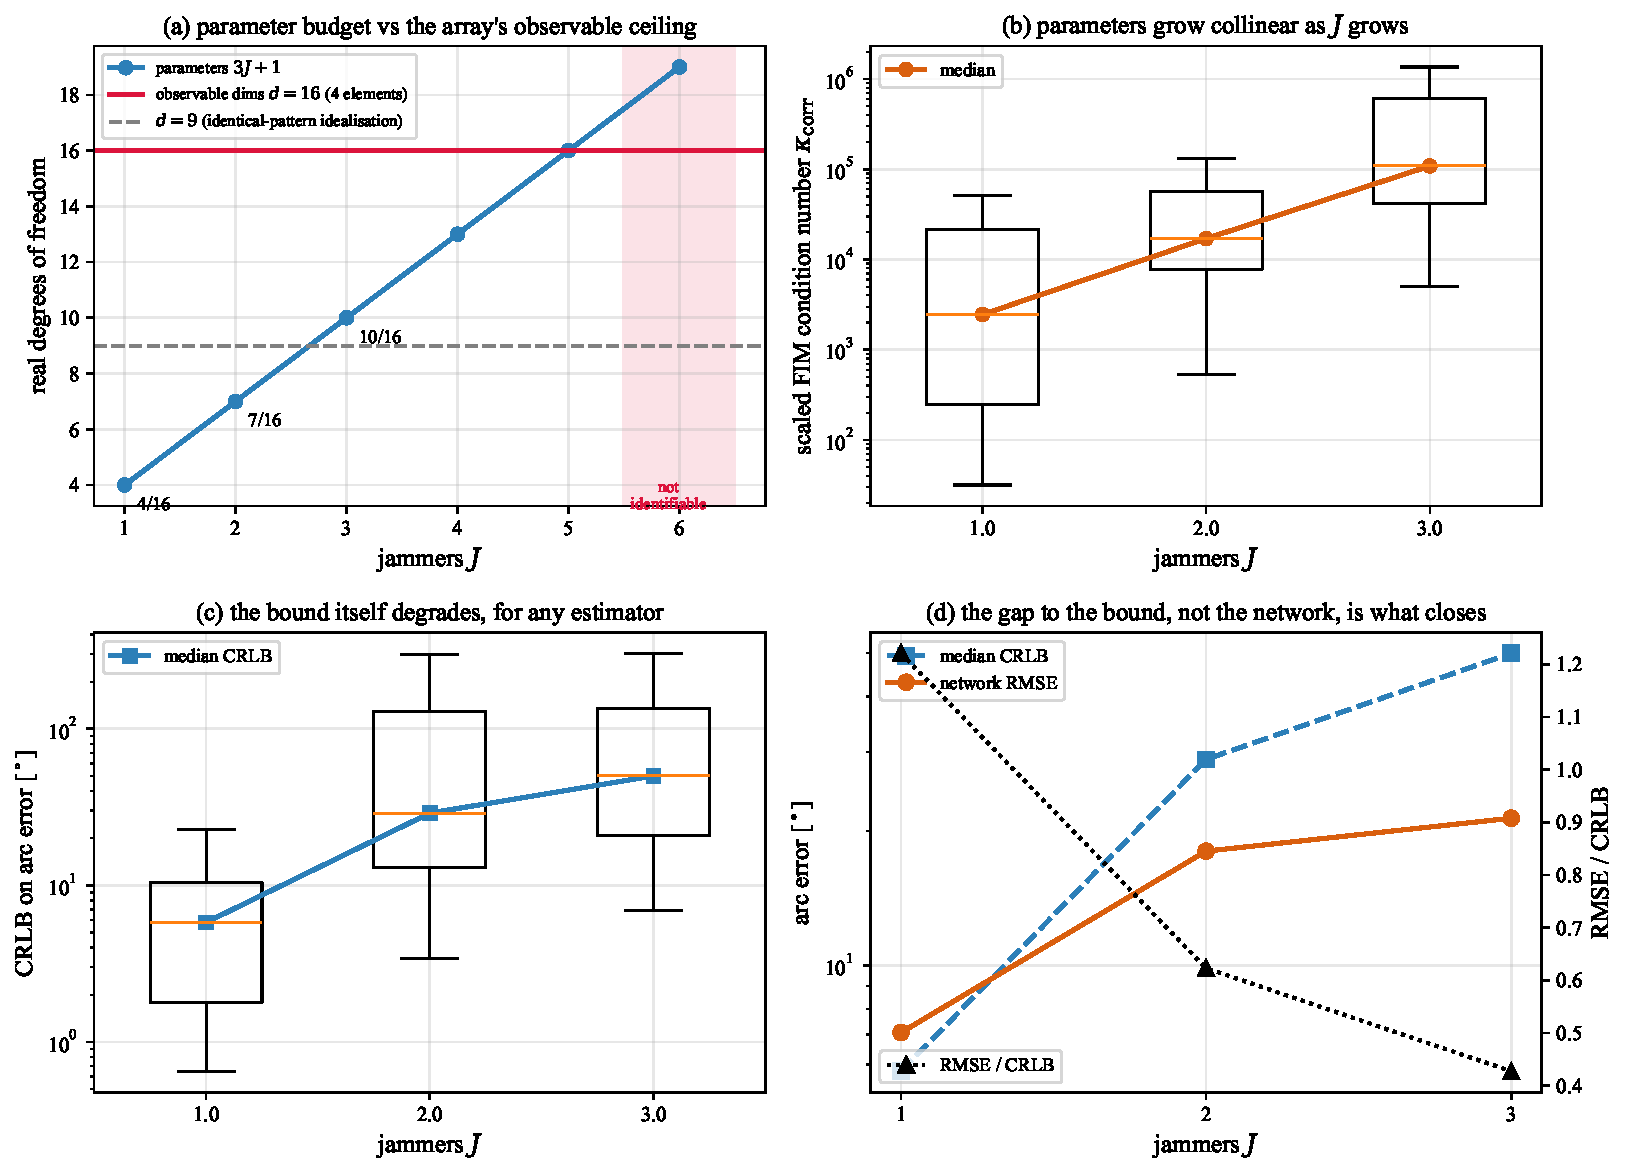
\includegraphics[width=\columnwidth]{phase3j_conditioning_vs_dof}
\caption{Conditioning of the power-only Fisher information and the resulting
bound, against the number of jammers (COND). The correlation-normalised
condition number of \eqref{eq:kappacorr} rises from $\kappaOneJ$ at $J = 1$ to
$\kappaThreeJ$ at $J = 3$, a factor of $\kappaGrowth$, and the median
per-scene arc bound rises from $\crbMedOneJ\degs$ to $\crbMedThreeJ\degs$, a
factor of $\crbGrowth$. The estimator's RMSE over the same span grows by only
$\netRmseGrowth$; the gap is not efficiency but bias, as
Section~\ref{sec:single:bias} shows.}
\label{fig:cond}
\end{figure}

Equation~\eqref{eq:jmax} permits $J \le \jIdent$, and the array has
$\dObs$ dimensions to spend. Neither fact implies that a three-jammer scene is
comfortably observable, because identifiability is a statement about rank and
accuracy is a statement about conditioning. The two part company well before
the ceiling is reached, and Table~\ref{tab:cond} shows where.

Conditioning must be measured carefully here. The raw condition number of
$\mathbf{F}$ is meaningless for this problem: the $\ln\sigma_n^2$ column of the
Jacobian is of order $\sigma_n^2\sum_m\|\wv_m\|^2 \sim 10^{-14}$ while a jammer
power column at $35\dB$ is of order $10^{-11}$, and the quadratic form squares
that disparity, so $\mathbf{F}$ reports a condition number of
$\kappaRawOneJ$ even at $J = 1$ where nothing whatever is degenerate. That
number measures the choice of physical units, not the geometry. We therefore
report the condition number after symmetric diagonal scaling,
\begin{equation}
\kappa_{\mathrm{corr}}
= \kappa\big(\mathbf{D}^{-1/2}\,\mathbf{F}\,\mathbf{D}^{-1/2}\big),
\qquad
\mathbf{D} = \diag(\mathbf{F}),
\label{eq:kappacorr}
\end{equation}
which is the standard remedy for exactly this pathology and leaves a quantity
that responds to the correlation structure of the information rather than to
the units of its entries.

\begin{table}[!t]
\centering
\caption{Degrees of freedom, Fisher conditioning and the marginalised angular
bound as the jammer count grows. $\scenesPerRow$ scenes per row,
$\scenesTotal$ in total; no scene was rejected by the $\condLimit$ guard.}
\label{tab:cond}
\begin{tabular}{@{}cccccc@{}}
\toprule
$J$ & $3J{+}1$ & probes & used & $\kappa_{\mathrm{corr}}$ &
median $\CRB_{\mathrm{arc}}$ \\
\midrule
$1$ & $4$  & $8$  & $4/\dObs$  & $\kappaOneJ$   & $\crbMedOneJ\degs$ \\
$2$ & $7$  & $16$ & $7/\dObs$  & $\kappaTwoJ$   & $\crbMedTwoJ\degs$ \\
$3$ & $10$ & $24$ & $\dSpentThreeJ/\dObs$ & $\kappaThreeJ$ & $\crbMedThreeJ\degs$ \\
\bottomrule
\end{tabular}
\end{table}

The pattern is unambiguous. Going from one jammer to three, the number of
readings available actually \emph{triples}, from $\numProbes$ to $24$, because
one query is issued per jammer. Despite that, the scaled conditioning degrades
by $\kappaGrowth\times$ and the bound itself degrades by $\crbGrowth\times$,
from $\crbMedOneJ\degs$ to $\crbMedThreeJ\degs$. More measurements bought no
accuracy, exactly as Section~\ref{sec:bounds:ceiling} said they could not: the
readings are extra rows through the same $\dObs$-dimensional bottleneck, and
the scene is now asking $\dSpentThreeJ$ questions of it instead of $4$.

That the $\condLimit$ guard rejected $\nBad$ scenes out of $\scenesTotal$ is
the other half of the statement, and it is what makes the diagnosis specific.
The three-jammer Fisher matrix is not rank deficient; the parameters remain
formally identifiable. What has happened is that the information has become
strongly correlated across parameters, so that recovering any one direction
requires unpicking it from the others. This is a conditioning loss, and the
distinction is practical rather than semantic: a conditioning loss on a
full-rank problem cannot be repaired by a better read-out of the same
$\numProbes$ numbers, however sophisticated. It is repaired by adding
independent information --- more elements, hence a larger $\dObs$, or
independent looks across time or frequency. A stronger estimator is not the
missing ingredient, because the ingredient that is missing is not in the
measurement.

This sets the expectation the estimator must be judged against, and it is a
deliberately uncomfortable one: the bound says a
three-jammer scene on this aperture is roughly $\crbGrowth\times$ harder than a
single-jammer scene. How the trained estimator actually degrades over the same
range, and why its error ratio against this bound behaves differently on
well- and ill-conditioned geometries, is taken up with the measured results.

%==============================================================================
\section{Estimator Architecture}
\label{sec:arch}
%==============================================================================

The estimator receives exactly what the front end produces: the eight scalars
of one sector query, plus the sector index. Its design is dictated by the two
structural facts established above --- that the probes are notches read by an
$\argmin$, and that the subsector centres are the only fixed directional
landmarks available. The network is therefore built as a geometric anchor that
a learned refiner corrects, rather than as a generic regressor from
$\mathbb{R}^{8}$ to two angles.

\subsection{The Geometric Anchor}
\label{sec:arch:anchor}

The first branch converts the probe vector into a set of non-negative weights
over the $\numProbes$ subsectors of the queried sector. A small
normalise--project--softmax stack maps $\pv$ to $\mathbf{a} \in \Delta^{7}$,
and the anchor direction is read off as the corresponding convex combination
of the subsector-centre encodings,
\begin{equation}
\begin{split}
\mathbf{g}_0 &= \sum_{m=1}^{\numProbes} a_m\, \mathbf{e}(\mathbf{c}_{s,m}), \\
\mathbf{e}(\theta,\phi) &=
\big[\cos\theta,\ \sin\theta,\ \cos\phi,\ \sin\phi\big]^{\Tr},
\end{split}
\label{eq:anchor}
\end{equation}
the $\centerDim$-component trigonometric encoding being used in place of the
raw angle pair so that azimuth carries no branch cut. Equation
\eqref{eq:anchor} is a differentiable soft $\argmin$: it is the learned
counterpart of the bare $\argmin$ read-out that already recovers the occupied
subsector $\argminExact\%$ of the time, and it inherits that read-out's
robustness rather than having to rediscover it.

A convex combination, however, cannot leave the convex hull of the
$\numProbes$ centres, so \eqref{eq:anchor} alone can never return a direction
near a sector edge. A second small head reads $\pv$ and emits an additive
offset that releases the anchor from the hull,
$\mathbf{g} = \mathbf{g}_0 + \mathbf{h}(\pv)$, with $\mathbf{h}$
\emph{zero-initialised}. The initialisation matters: at the start of training
the model is exactly the soft $\argmin$ of \eqref{eq:anchor}, and every
departure from it is something the data paid for.

\subsection{The Attention Refiner}
\label{sec:arch:attn}

The anchor is accurate to roughly a subsector. Resolving within a subsector
requires reading the relative depths of all eight notches jointly, which is a
comparison task, so the second branch is an attention block. The probe vector
is presented as a sequence of $\numTokens$ tokens of width $\embedDim$: one
token carrying the anchor encoding, one carrying the logarithm of the scale
removed when $\pv$ was normalised, and one per probe reading. A single
$\numHeads$-head self-attention layer lets every probe token be interpreted
relative to the others, which is precisely the operation a notch codebook
demands, since the informative quantity is a \emph{contrast} between readings
and not any reading on its own.

The separate scale token is deliberate. Normalising $\pv$ is necessary --- the
absolute received power spans the $\jnrLo$--$\jnrHi\dB$ range and would
otherwise dominate the input --- but it is not harmless, because the noise
term in \eqref{eq:measnoise} is referenced to the scan mean, so the scale
carries information about how trustworthy the shape is. Supplying it as its
own token preserves that information without letting it swamp the shape.

\subsection{Hemisphere by Construction}
\label{sec:arch:constraint}

The refiner emits a three-component correction, and the way it is applied is
the one architectural choice that removes an entire class of failure. Rather
than correcting $\theta$ additively and repairing the result, the correction
is applied in the \emph{logit of $\cos\theta$},
\begin{equation}
\cos\hat\theta
= \sigma\!\Big(
\operatorname{logit}\big(\cos\theta_{\mathbf{g}}\big) + \Delta_\theta
\Big),
\qquad
\sigma(x) = \frac{1}{1+e^{-x}},
\label{eq:thetalogit}
\end{equation}
so that $\cos\hat\theta \in (0,1)$ and hence
$\hat\theta \in (0\degs, 90\degs)$ for \emph{any} real $\Delta_\theta$. The
azimuth correction is a residual on the unit circle, renormalised after
addition. The upper hemisphere is thus enforced by the parameterisation
itself: there is no folding, no clipping and no angle wrapping anywhere in the
model, and consequently no discontinuity for the optimiser to fight. The
residual structure survives intact, merely expressed in logit space. That this
is not a vacuous guarantee is visible in the predictions, which span
$\thetaPredLo\degs$ to $\thetaPredHi\degs$ without a single folded output.

The whole model is $\modelParams$ parameters. Inference is one forward pass
with no iteration, no search and no matrix inversion, so the deployed latency
is set by the $0.40\,\mathrm{s}$ probe scan of Section~\ref{sec:model:stats}
and not by the estimator.

%==============================================================================
\section{Single-Jammer Accuracy and the Anatomy of the Error}
\label{sec:single}
%==============================================================================

\subsection{Accuracy}
\label{sec:single:acc}

Over $\phOneN$ single-jammer scenes with $\JNR$ drawn across the full
$\jnrLo$--$\jnrHi\dB$ range, the arc error \eqref{eq:arcerr} has median
$\netArcPfifty\degs$, ninetieth percentile $\netArcPninety\degs$ and
$\RMSE$ $\netArcRmse\degs$. Resolved into components, the zenith error is
$\netZenPfifty\degs$ at the median and $\netZenPninety\degs$ at the ninetieth
percentile, the azimuth error $\netAziPfifty\degs$ and
$\netAziPninety\degs$.

The gap between the median and the $\RMSE$ --- roughly a factor of two --- is
the first thing to notice, and it is why both are quoted. The error
distribution is not Gaussian but tail-dominated: most scenes are resolved to
a few degrees, and a minority in which the notch carries little information
are resolved very poorly and dominate any second-moment summary.
Figure~\ref{fig:cdf} shows the distribution directly, and an $\RMSE$ quoted
alone would misrepresent it in either direction depending on the reader's
assumption.

\begin{figure}[!t]
\centering
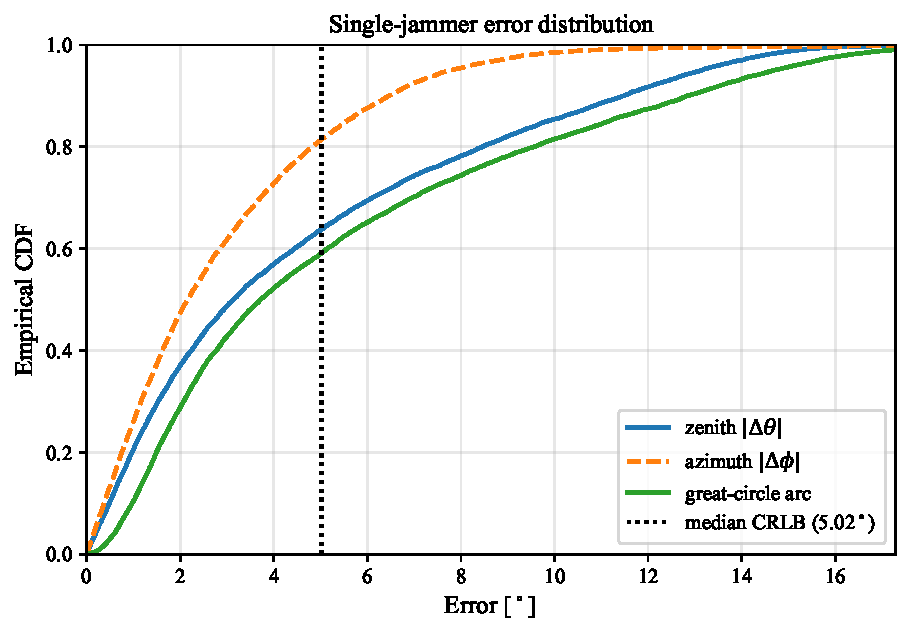
\includegraphics[width=\columnwidth]{phase1_error_cdf}
\caption{Cumulative distribution of the single-jammer arc error over
$\phOneN$ scenes. The distribution is tail-dominated: the median is
$\netArcPfifty\degs$ but the $\RMSE$ is $\netArcRmse\degs$, so the two
summaries answer different questions and both are reported.}
\label{fig:cdf}
\end{figure}

\subsection{Efficiency Is a Function of Geometry, Not a Number}
\label{sec:single:eff}

\begin{figure}[!t]
\centering
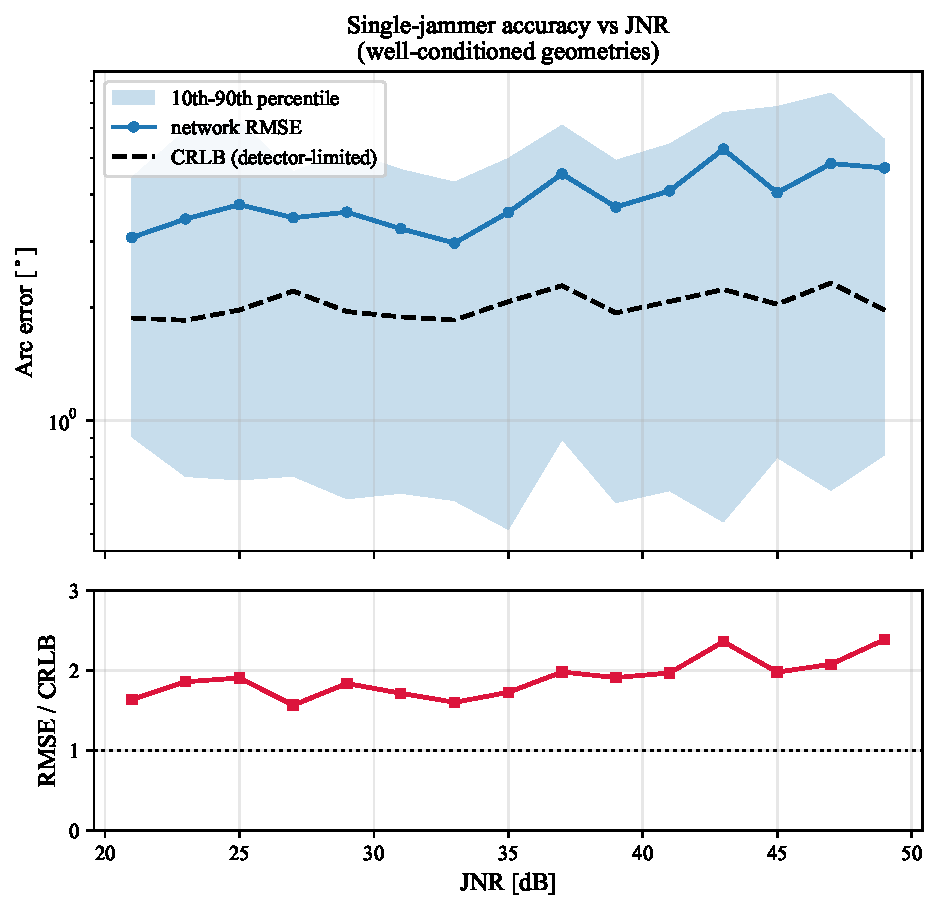
\includegraphics[width=\columnwidth]{phase1_jnr_efficiency}
\caption{Random-DoA sweep over $\phOneN$ scenes (PH1). Accuracy is flat in
jammer-to-noise ratio across the whole generator range,
$\netRmseJnrLo\degs$ RMSE in the lowest decade against $\netRmseJnrHi\degs$ in
the highest, because a notch codebook reports a ratio of powers and the ratio
is insensitive to the common scale. The ratio $\RMSE/\CRB$, by contrast, is
strongly geometry-dependent: $\effWell$ on the well-conditioned half of the
scenes and $\effIll$ on the ill-conditioned half. The aggregate $\effAgg$ is
an average of two populations that behave oppositely and is not an efficiency.}
\label{fig:eff}
\end{figure}

Comparing this against the bound of Section~\ref{sec:bounds} requires care,
because the bound itself varies by more than an order of magnitude across the
hemisphere: over $\crbNbounds$ scenes its median is $\crbPhaseOneMed\degs$
with a tenth percentile of $\crbPhaseOnePten\degs$ and a ninetieth of
$\crbPhaseOnePninety\degs$. Aggregating in quadrature gives an
RMS bound of $\crbRms\degs$ and an overall ratio of $\effAgg\times$. We
decline to report that number as a result. A single ratio formed across a
population whose bound spans an order of magnitude is an average of two
qualitatively different behaviours, and it conceals both of them.

Splitting the population at its own median bound separates them cleanly. On
the well-conditioned half the network achieves $\effWellRmse\degs$ against a
bound of $\effWellCrb\degs$, a ratio of $\effWell\times$; on the
ill-conditioned half it achieves $\effIllRmse\degs$ against
$\effIllCrb\degs$, a ratio of $\effIll\times$. The estimator is thus a
factor of two from efficient where the geometry is informative, and sits
\emph{below} the unbiased bound where it is not. The second number is the one
that requires an explanation rather than a celebration, and
Section~\ref{sec:single:bias} provides it.

One prediction of Section~\ref{sec:bounds:predict} can be checked in passing.
The bound was shown to be independent of $\JNR$; measured on this population
it is $\crbJnrLo\degs$ below $30\dB$ and $\crbJnrHi\degs$ above $40\dB$. The
network tracks that flatness, at $\netRmseJnrLo\degs$ and
$\netRmseJnrHi\degs$ respectively. Neither the bound nor the estimator
improves with jammer power, which is the signature of a front end whose
accuracy floor is relative rather than absolute.

\subsection{Separating Bias From Variance Exactly}
\label{sec:single:bias}

A ratio below unity against an unbiased bound admits only two explanations:
the bound is wrong, or the estimator is biased. Section~\ref{sec:bounds:verify}
has already closed off the first. Establishing the second requires separating
bias from scatter, and the sweep of Section~\ref{sec:single:acc} cannot do it,
because the direction changes on every scene, so systematic and random error
are hopelessly entangled.

We therefore ran a second, differently designed experiment. The hemisphere was
sampled on a grid of $\fdRings$ zenith rings by $\fdSpokes$ azimuth spokes,
giving $\fdDirs$ directions, and at each direction the DoA was held
\emph{fixed} while $\fdTrials$ independent noise realisations were drawn at
$\JNR = \fdJnr\dB$ --- $\fdQueries$ queries in total. Because the truth is
constant within a direction, the decomposition
\begin{equation}
\mathrm{MSE}(\mathbf{c})
= \big\|\mathbf{b}(\mathbf{c})\big\|^2 + s(\mathbf{c})^2
\label{eq:biasvar}
\end{equation}
into a bias vector $\mathbf{b}$ and a scatter $s$ holds \emph{exactly} rather
than approximately, and each can be measured without reference to the other.

Aggregated over the grid, the median bias magnitude is $\fdBiasMed\degs$
against a median scatter of $\fdScatMed\degs$, for a median per-direction
$\RMSE$ of $\fdRmseMed\degs$ and a bias fraction of $\fdBiasFrac$. The error
of this estimator is predominantly \emph{systematic}, which already tells us
that the unbiased bound is not the natural yardstick for it.

\begin{table}[!t]
\centering
\caption{Fixed-DoA bias/variance decomposition, split at this experiment's own
median bound ($\fdSplit\degs$). All quantities in degrees except the last two
columns. Between the halves the bias grows $\fdBiasGrowth\times$ while the
scatter moves by $\fdScatGrowth\%$: the degradation is almost entirely
systematic.}
\label{tab:biasvar}
\small
\setlength{\tabcolsep}{4pt}
\begin{tabular}{@{}lccccc@{}}
\toprule
Half & $\RMSE$ & $\|\mathbf{b}\|$ & $s$ & bias frac. & $\RMSE/\CRB$ \\
\midrule
Well-cond. & $\fdWellRmse$ & $\fdWellBias$ & $\fdWellScat$ & $\fdWellFrac$ & $\fdWellEff$ \\
Ill-cond.  & $\fdIllRmse$  & $\fdIllBias$  & $\fdIllScat$  & $\fdIllFrac$  & $\fdIllEff$ \\
\bottomrule
\end{tabular}
\end{table}

Table~\ref{tab:biasvar} is the decisive measurement. Moving from the
well-conditioned to the ill-conditioned half, the bias magnitude grows from
$\fdWellBias\degs$ to $\fdIllBias\degs$ --- a factor of
$\fdBiasGrowth\times$ --- while the scatter moves only from
$\fdWellScat\degs$ to $\fdIllScat\degs$, some $\fdScatGrowth\%$. The random
part of the error is essentially constant across the hemisphere; everything
that degrades is systematic. Correspondingly the bias fraction rises from
$\fdWellFrac$ to $\fdIllFrac$, and the ratio against the bound falls from
$\fdWellEff\times$ to $\fdIllEff\times$.

Of the $\fdDirs$ directions, $\fdSubN$ --- $\fdSubPct\%$ --- have an $\RMSE$
below their own bound. Their median bias fraction is $\fdSubFrac$ against
$\fdRestFrac$ for the rest. The sub-bound directions are precisely the
bias-dominated ones. This is the expected behaviour of an estimator that
trades bias for variance where the geometry carries little information, and it
is not superefficiency: a genuinely unbiased estimator cannot sit below the
bound, and this one is demonstrably not unbiased. We therefore make no
efficiency claim on the ill-conditioned half.

It is worth stating plainly that this experiment and the sweep of
Section~\ref{sec:single:eff} are independent, with different designs,
different sample counts and different median bounds --- $\fdSplit\degs$ here
against $\crbPhaseOneMed\degs$ there. Their conditioning splits are therefore
not the same numbers and should not be quoted as such: the fixed-DoA
experiment gives $\fdWellEff\times$ and $\fdIllEff\times$, the random-DoA
sweep $\effWell\times$ and $\effIll\times$. That two differently constructed
experiments produce the same qualitative split --- comfortably above the bound
where the geometry is good, below it where the geometry is poor --- is the
point, and it is stronger evidence than either alone.

\subsection{Where the Bias Points}
\label{sec:single:where}

A bias that merely existed would be a nuisance; this one has a direction, and
the direction identifies the mechanism. For each grid point we compared the
measured bias vector against the bearing from that point to its sector centre.
The magnitude-weighted mean cosine is $+\fdBiasCos$, and the
magnitude-weighted probability that the bias points inward is $\fdPin$
($\fdPinUnw$ unweighted). The bias is aimed at the sector centres --- which
are exactly the fixed landmarks of \eqref{eq:anchor}.

Figures~\ref{fig:biasvar} and~\ref{fig:spatialmap} show this: the first
separates the two error components direction by direction, the second places
them on the hemisphere. The mechanism is the anchor's
fallback: when the notch is shallow and the probe contrast carries little
information, the softmax of Section~\ref{sec:arch:anchor} spreads its mass
over several subsectors, and a spread convex combination necessarily retreats
toward the interior of the hull. The learned hull offset compensates only
partially. The estimator's failure mode is therefore not noise amplification
but a graceful collapse onto its own prior, which is also why the scatter
barely moves while the bias grows.

This is most pronounced at high zenith angles, where the bias exceeds the
scatter several-fold and the ratio against the bound is at its lowest. Two
cautions attach to reading that trend off the elevation axis. First, as noted
in Section~\ref{sec:model:sectors}, $\theta = \elevSplit\degs$ is
simultaneously the equal-solid-angle split and a sector boundary, so a step
across it is the partition showing through rather than a property of the sky.
Second, the bound itself grows steeply toward the horizon, so a falling ratio
there reflects a rising denominator as much as a rising numerator.

\begin{figure*}[!t]
\centering
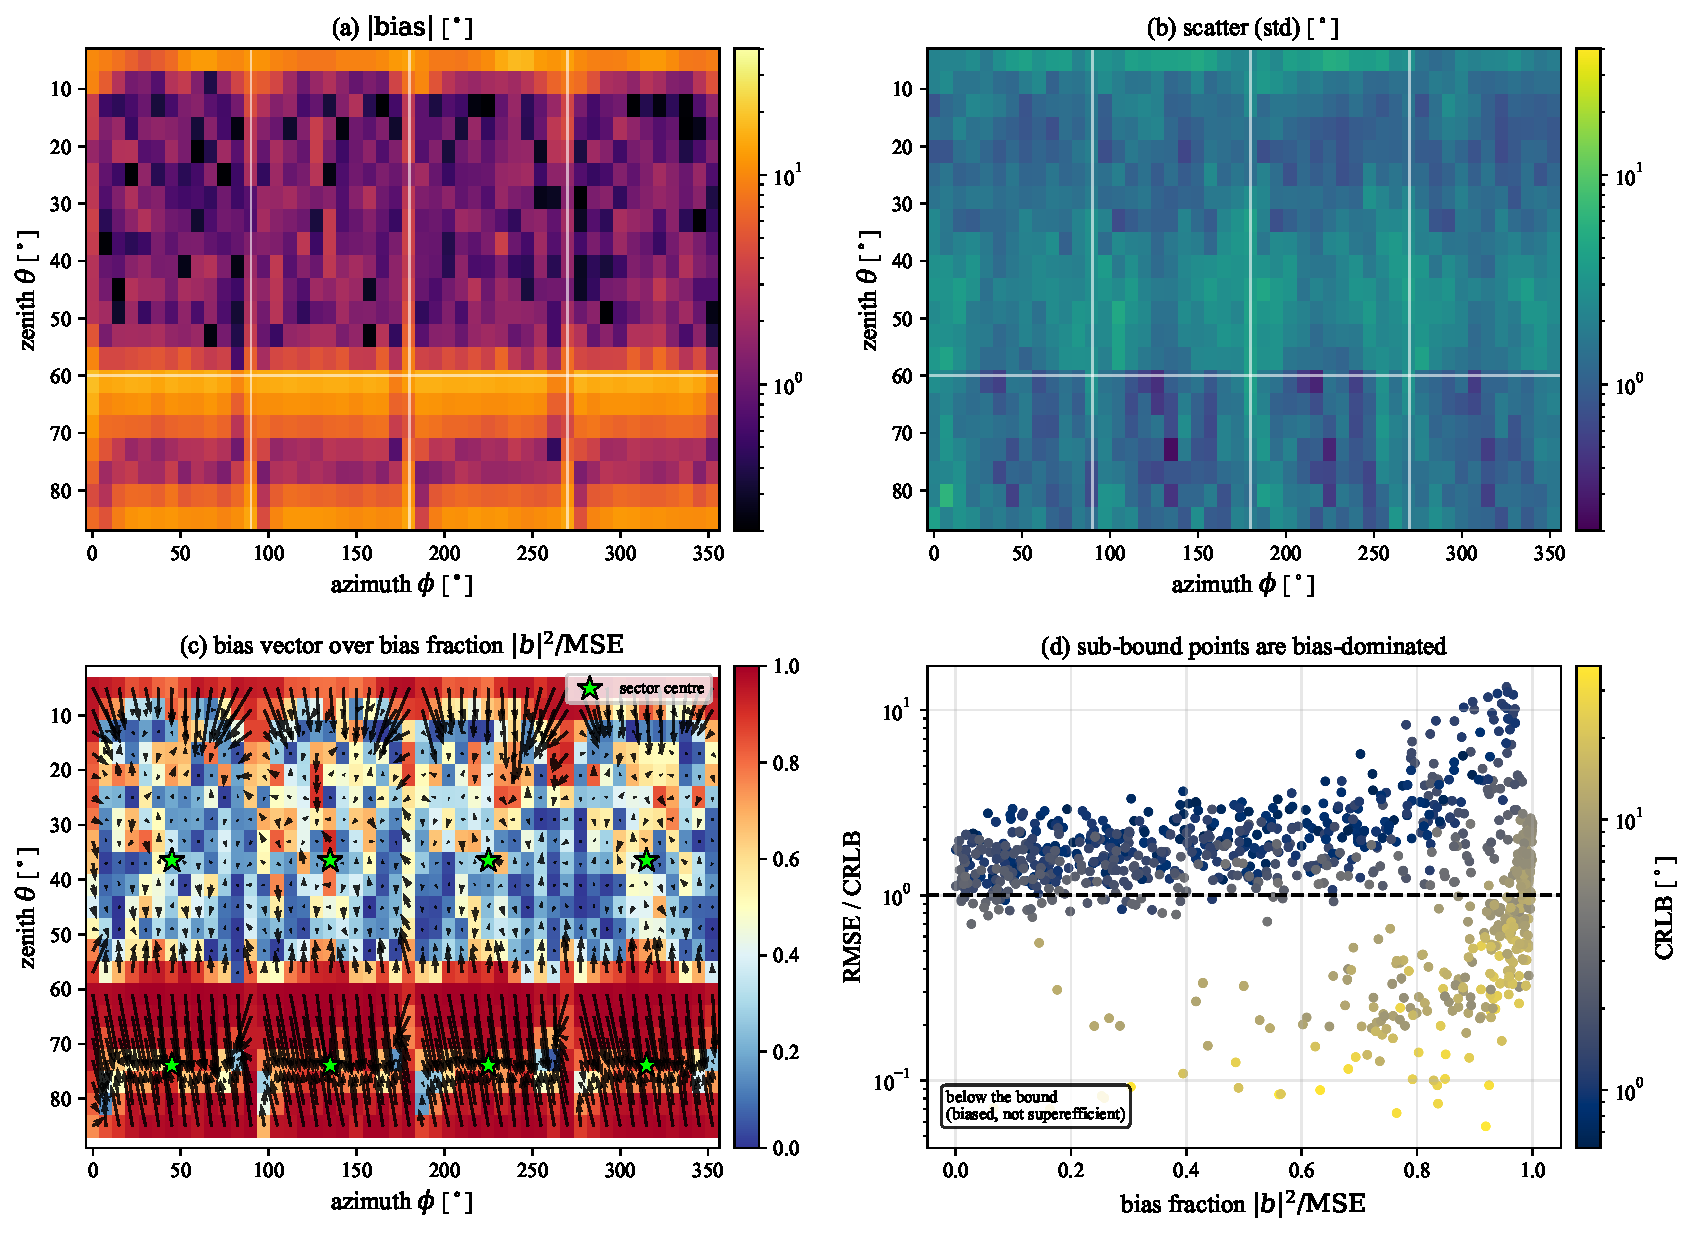
\includegraphics[width=\textwidth]{phase1_bias_variance}
\caption{The fixed-DoA experiment: the error at each of the $\fdDirs$
directions separated into its systematic and random parts according to
\eqref{eq:biasvar}. The bias grows $\fdBiasGrowth\times$ between the
conditioning halves while the scatter moves only $\fdScatGrowth\%$, which is
what makes the sub-bound cells bias-dominated rather than efficient. The
sub-panels are internal to the figure.}
\label{fig:biasvar}
\end{figure*}

\begin{figure*}[!t]
\centering
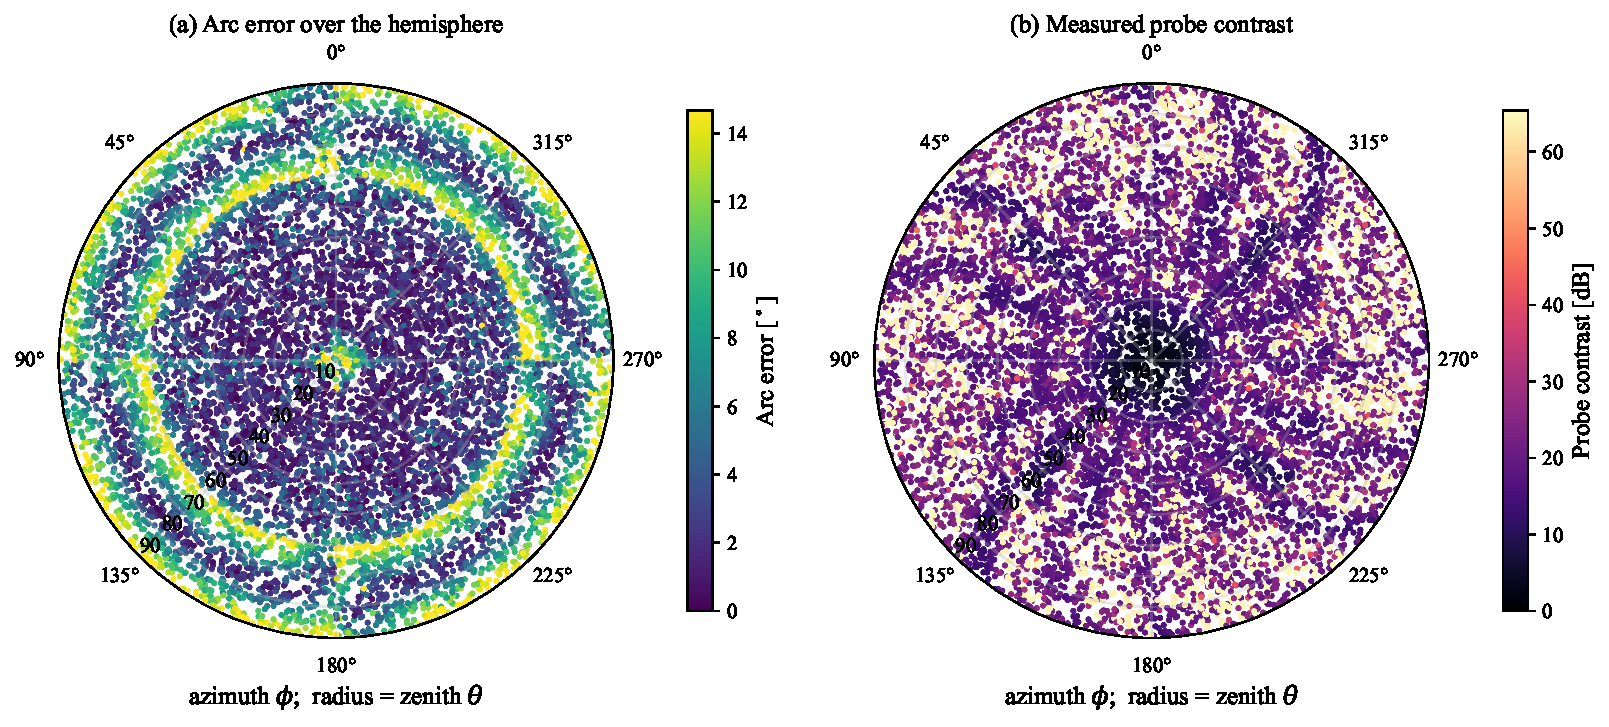
\includegraphics[width=\textwidth]{phase1_spatial_map}
\caption{The same fixed-DoA errors placed on the hemisphere. The bias vectors
point inward, toward the subsector centres from which the anchor of
\eqref{eq:anchor} is built: the magnitude-weighted probability of pointing
inward is $\fdPin$ and the magnitude-weighted mean cosine is $+\fdBiasCos$.
Structure along $\theta = \elevSplit\degs$ is partly geometric and partly the
codebook band boundary, and the two cannot be separated with a single
codebook.}
\label{fig:spatialmap}
\end{figure*}

%==============================================================================
\subsection{Each Stage Earns Its Place, but Not Equally}
\label{sec:single:stages}

Because the estimate is the sum of an analytic anchor, a learned offset applied
to that anchor and a transformer correction, the output can be recomposed one
stage at a time and every partial sum scored against the same truth. Over
$\decompN$ single-jammer queries the anchor alone --- the soft $\argmin$ of
\eqref{eq:anchor} with the learned offsets held at zero --- reaches a median
arc error of $\hullPfifty\degs$ and a ninetieth percentile of
$\hullPninety\degs$. That is far better than chance, and it is a direct
confirmation of the claim made in Section~\ref{sec:model:probes}: the minimum
of a notch codebook is a usable direction estimator in its own right, before
any learning at all. Enabling the learned offset moves the median to
$\hullOffPfifty\degs$, an improvement of $\recSixMove\degs$, while the tail
gets marginally worse, $\hullOffPninety\degs$ against $\hullPninety\degs$. The
transformer correction then brings the median to $\netArcPfifty\degs$, a
further $\transformerAdd\degs$, and the ninetieth percentile to
$\netArcPninety\degs$.

The honest reading of Fig.~\ref{fig:decomp} is that two of the three stages
carry the result and the third is close to idle. The anchor contributes the
coarse, geometry-bound estimate that keeps the answer inside the queried
sector. The refiner contributes the interpolation between subsector centres
that converts a $\hullPfifty\degs$ answer into a $\netArcPfifty\degs$ one, and
it is where essentially all of the accuracy of the method resides. The learned
offset on the anchor contributes little enough that it could be deleted for
well under a degree of median error. We report that rather than suppress it for
two reasons. It localises the contribution of learning in the refiner, which is
the claim the architecture was designed to test. And it identifies the floor
that the system falls back to when the probe vector stops being informative ---
a floor set by the fixed sector geometry, not by the network --- which is
exactly the behaviour observed in Section~\ref{sec:dynrange}.

\begin{figure}[!t]
\centering
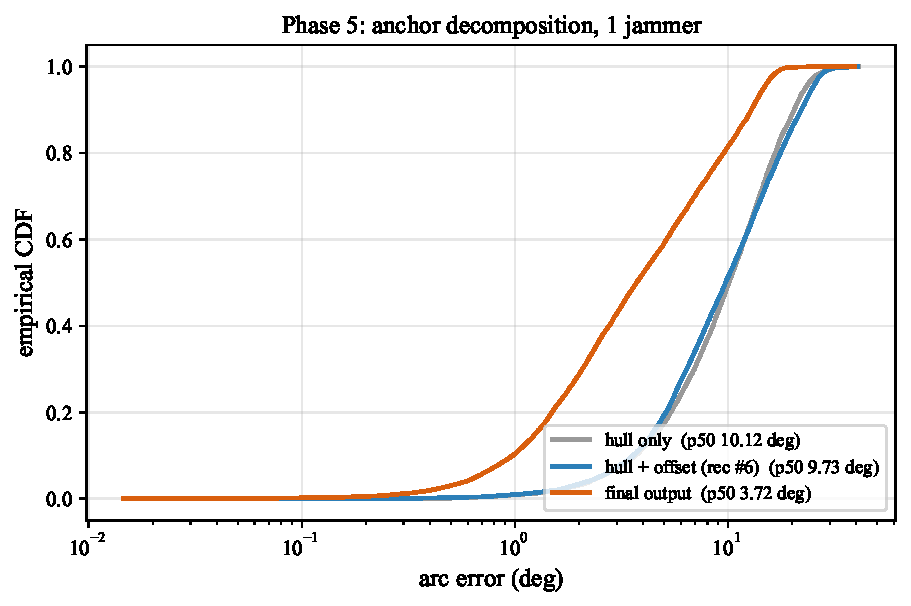
\includegraphics[width=\columnwidth]{phase5_decomposition}
\caption{Stage-by-stage recomposition of the estimator over $\decompN$
single-jammer queries (PH5). Anchor alone, anchor plus learned offset, and the
full output are scored against the same truths. The recomposition is exact:
summing the stages reproduces the forward pass to machine precision, so the
comparison is an attribution and not an ablation retrained per stage.}
\label{fig:decomp}
\end{figure}

\section{Multiple Jammers: Degradation and Resolvability}
\label{sec:multi}

Section~\ref{sec:bounds:ceiling} predicted that this array runs out of
observable dimensions quickly, and Section~\ref{sec:bounds:cond} showed the
Fisher information becoming badly scaled well before the count is exhausted.
This section measures what that costs. Two experiments are reported: a
degradation sweep across $J \in \{1, 2, 3\}$, and a dedicated two-jammer
resolvability study that asks not how large the errors are but whether the two
directions are separated at all.

\subsection{How the Error Grows with the Jammer Count}
\label{sec:multi:grow}

Table~\ref{tab:multij} reports per-jammer arc error against $J$. Errors are
matched to truths by the Hungarian assignment described in
Section~\ref{sec:model:problem}, so a permutation is never counted as an error,
and the estimate count is $J$ times the scene count. The median roughly
triples from $J = 1$ to $J = 2$ and then grows only modestly to $J = 3$, while
the ninetieth percentile grows more evenly. The shape matters more than the
magnitudes: the penalty for the second jammer is much larger than the penalty
for the third.

\begin{table}[!t]
\centering
\caption{Per-jammer arc error against the number of jammers, after Hungarian
matching (PH3J).}
\label{tab:multij}
\begin{tabular}{lrrrr}
\toprule
$J$ & estimates & $p_{50}$ ($\degs$) & $p_{90}$ ($\degs$) & RMSE ($\degs$) \\
\midrule
$1$ & $\phOneN$  & $\netArcPfifty$   & $\netArcPninety$   & $\netArcRmse$ \\
$2$ & $\jTwoN$   & $\jTwoPfifty$     & $\jTwoPninety$     & $\jTwoRmse$ \\
$3$ & $\jThreeN$ & $\jThreePfifty$   & $\jThreePninety$   & $\jThreeRmse$ \\
\bottomrule
\end{tabular}
\end{table}

That shape is the signature of an estimator leaning on prior geometry. The
bound behaves quite differently, as Fig.~\ref{fig:cond} showed: the median
per-scene bound degrades by a factor of $\crbGrowth$ between $J = 1$ and
$J = 3$, while the measured RMSE degrades by only $\netRmseGrowth$. A reader
could be tempted to read the difference as increasing efficiency. It is not.
The bound is the right yardstick only for an unbiased estimator, and
Section~\ref{sec:single:bias} established by direct measurement that this
estimator is biased toward subsector centres. As the scene becomes
information-poor the estimate retreats toward that fixed geometry, which limits
the error growth precisely because it stops tracking the data. Nothing here
beats the Cram\'er--Rao bound; the estimator simply ceases to be the kind of
estimator the bound describes.

\begin{figure}[!t]
\centering
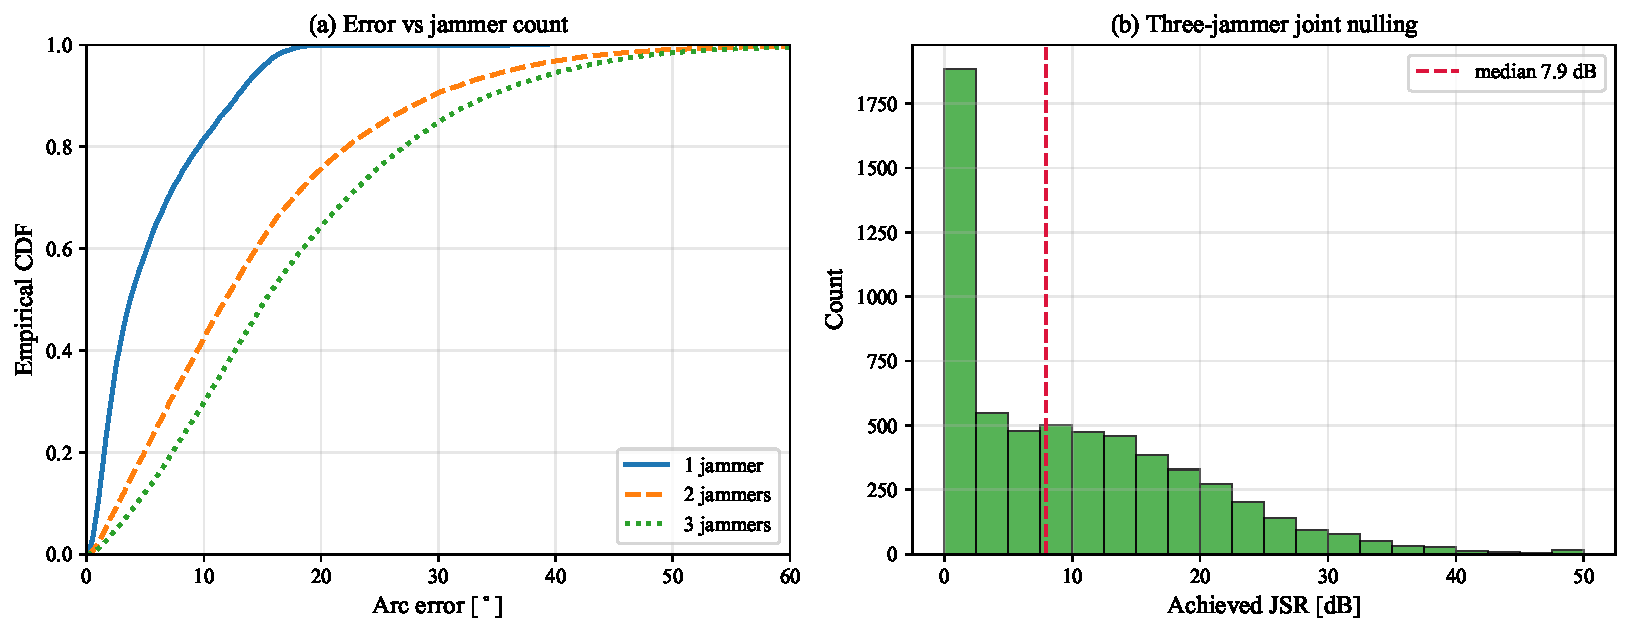
\includegraphics[width=\columnwidth]{phase3j_summary}
\caption{Multi-jammer degradation (PH3J). Error distributions for
$J \in \{1, 2, 3\}$ on common axes, together with the joint-nulling outcome at
$J = 3$. With $J = 3$ nulls demanded of an $\numElem$-element array only a
single spatial degree of freedom is left over, so even exact directions would
purchase limited quiescent gain; the $J = 3$ figures should be read as
feasibility numbers rather than as an operating point.}
\label{fig:multij}
\end{figure}

At $J = 3$ the notion of a per-jammer error becomes strained, because the three
estimates are frequently not in one-to-one correspondence with the three
jammers in any useful sense. Requiring all three estimates to fall within a
third of the minimum pairwise separation, the criterion used throughout this
paper, succeeds in $\resThreeJ\%$ of scenes, even though the median closest
pair in those scenes is $\closestPairMed\degs$ apart --- a wide separation by
the standards of a $\apertureLambda\lambda$ aperture. Ten of the $\dObs$
observable dimensions are consumed at $J = 3$ and the Fisher information is
badly scaled, so this is the array speaking rather than the estimator.

\subsection{Resolving Two Jammers}
\label{sec:multi:res}

A separate experiment isolates the two-jammer case, where the question is
sharper: does the estimator return two distinct directions, or does it collapse
onto the midpoint? Over $\phTwoN$ scenes, both directions land within a third
of the true separation in $\resRate\%$ of cases. Two diagnostics confirm that
this is genuine resolution. First, the Hungarian matching swaps the two labels
in only $\swapRate\%$ of scenes, so the pairing is essentially never ambiguous.
Second, the median ratio of arc error to true separation is $\errOverSep$;
collapse onto the midpoint of the pair would drive that ratio to $0.5$, and a
value near a sixth of that is not consistent with systematic collapse.

Resolution is governed by separation in the way spatial processing always
predicts, and Fig.~\ref{fig:res} shows the trend. In the $15$--$20\degs$
separation bin only $\resSepLo\%$ of pairs are resolved; by the
$85$--$90\degs$ bin the rate is $\resSepHi\%$, with the fifty-percent crossing
near $\resCross\degs$. For an aperture of $\apertureLambda\lambda$ that
crossing is unsurprising, and it is worth stating plainly that the useful
two-jammer regime for this antenna is the widely separated one.

\begin{figure}[!t]
\centering
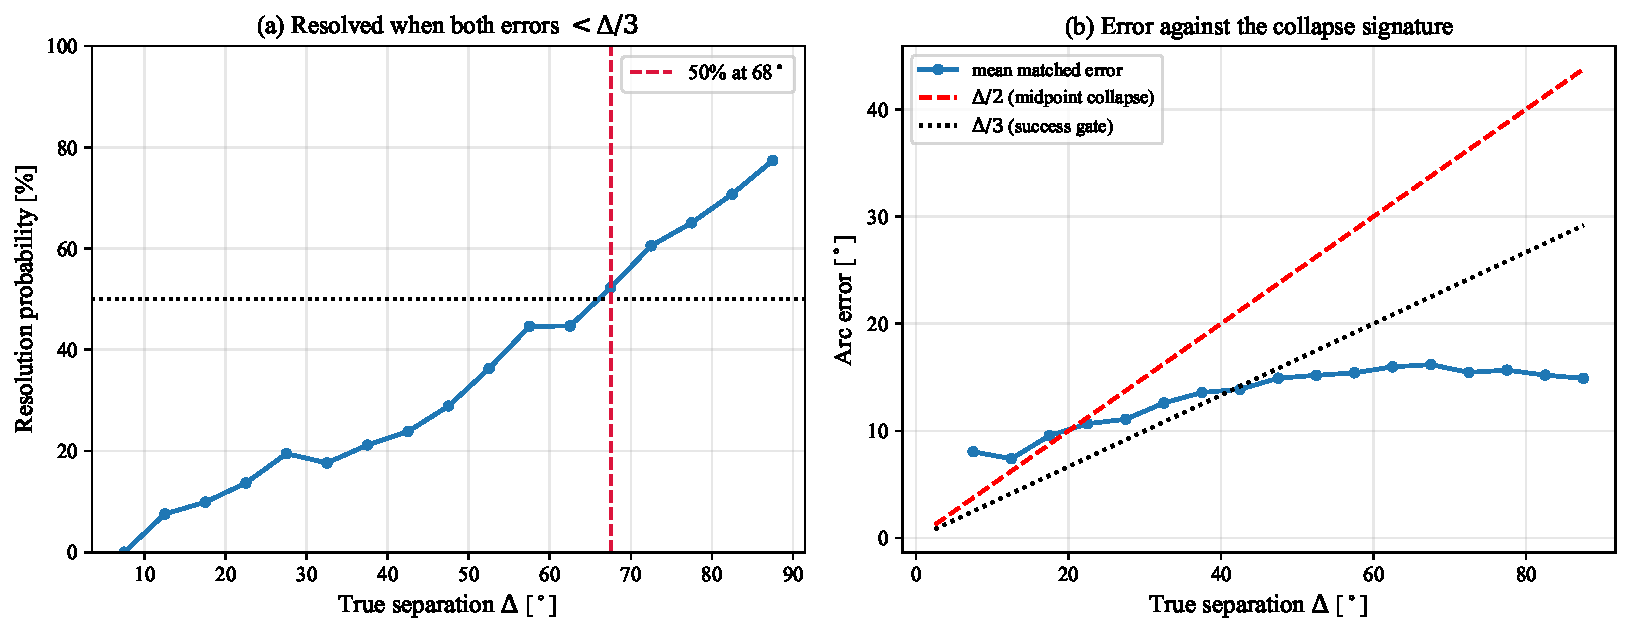
\includegraphics[width=\columnwidth]{phase2_resolution}
\caption{Two-jammer resolvability over $\phTwoN$ scenes (PH2). Resolution rate
against true angular separation, with the per-bin sample counts; the
fifty-percent crossing falls near $\resCross\degs$. Resolution requires both
estimates to lie within a third of the true separation.}
\label{fig:res}
\end{figure}

Power disparity matters less than separation, which is the more interesting
result. Splitting the same scenes by the jammer-to-noise difference, pairs
within $5\dB$ of each other resolve at $\resNearEq\%$ ($n = \nNearEq$) and
pairs more than $15\dB$ apart at $\resDisp\%$ ($n = \nDisp$). The penalty for a
strong jammer masking a weak one is real but modest, roughly eight points,
against the nearly eightfold swing produced by separation alone. The reason is
the notch codebook: because each probe suppresses its own centre, a strong
jammer does not saturate the reading of the probe that is nulling it, and the
weak jammer's contribution survives in that reading. This is a genuine
advantage of a nulling probe set over a beam-forming one, and
Section~\ref{sec:dynrange} quantifies where it finally breaks down.

\section{Dynamic Range: the Dominant Failure Mode}
\label{sec:dynrange}

The two-jammer results above are aggregated over power disparity. Resolving
that axis explicitly gives the clearest single statement of this system's
limitation, and it is the one result that does not follow the theory of
Section~\ref{sec:bounds}.

Each of the $\phOneN$ two-jammer scenes contributes two target/interferer
assignments, giving $\drN$ evaluation points ordered by the target's
jammer-to-noise ratio minus the interferer's. The asymmetry is large.
Restricting to targets at least $10\dB$ weaker than their interferer, the RMSE
is $\drWeakRmse\degs$; restricting to targets at least $10\dB$ stronger, it is
$\drStrongRmse\degs$, a ratio of $\drAsym$. Across the extreme bands the
medians run from $\drBandLo\degs$ for the most disadvantaged targets to
$\drBandHi\degs$ for the most advantaged.

\begin{figure}[!t]
\centering
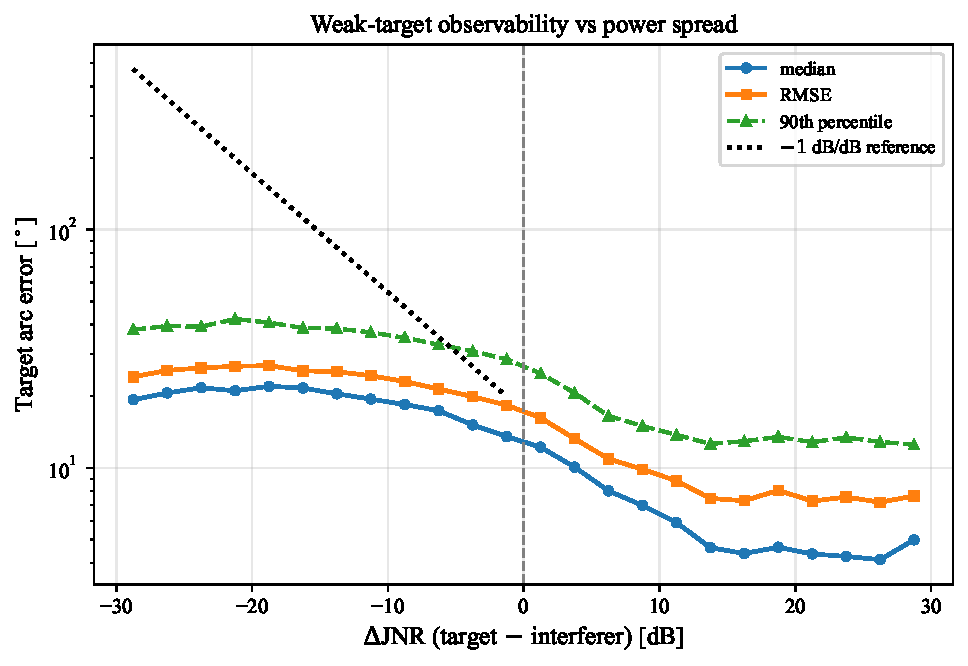
\includegraphics[width=\columnwidth]{phase3_5_dynamic_range}
\caption{Accuracy against target-to-interferer power ratio over $\drN$
evaluation points (PH35). The measured trend for disadvantaged targets is
$\drSlopeMeas\dB$ per $\dB$, against the $\drSlopePred$ predicted by the
weak-source law of Section~\ref{sec:bounds:predict}; instead of diverging, the
error saturates near $\drPlateau\degs$ beyond about $\drPlateauOnset\dB$ of
disparity.}
\label{fig:dynrange}
\end{figure}

The interesting part is that the estimator does not obey the law that governs
the bound. Section~\ref{sec:bounds:predict} showed that the per-scene bound for
a weak source degrades at very nearly $\weakSlopePred\dB$ per $\dB$ of
disparity, measured at $\weakSlopeMean\dB$ per $\dB$ over the sampled range,
which is to say the bound diverges as the target is buried. The network's error
does not diverge. Its measured trend over the disadvantaged bands is
$\drSlopeMeas\dB$ per $\dB$ --- flat to within the resolution of the
experiment, against $\drSlopePred$ predicted --- and beyond roughly
$\drPlateauOnset\dB$ of disparity the RMSE simply saturates at about
$\drPlateau\degs$ and stays there.

A saturating error is not a sign of strength, and it should not be read as one.
The plateau value is diagnostic. The hemisphere is divided into $\numSectors$
sectors, so a sector subtends a characteristic angular radius of about
$\sectorRadius\degs$, while a subsector subtends about
$\subsectorRadius\degs$. The observed plateau of $\drPlateau\degs$ sits at the
sector scale, not the subsector scale, which is what one expects of an
estimator that has fallen back on its coarsest prior. This is precisely the
mechanism identified in Section~\ref{sec:single:stages}: when the probe vector
carries no usable information about a buried target, the output reverts to the
anchor, and the anchor can be no better than the geometry it is built from. The
estimator therefore fails gracefully rather than catastrophically, returning a
sector-scale guess instead of a divergent one, but a sector-scale guess is not
a detection. Any deployment that must find weak emitters alongside strong ones
needs either a deeper codebook or a second look with the strong jammer already
nulled.

\begin{figure}[!t]
\centering
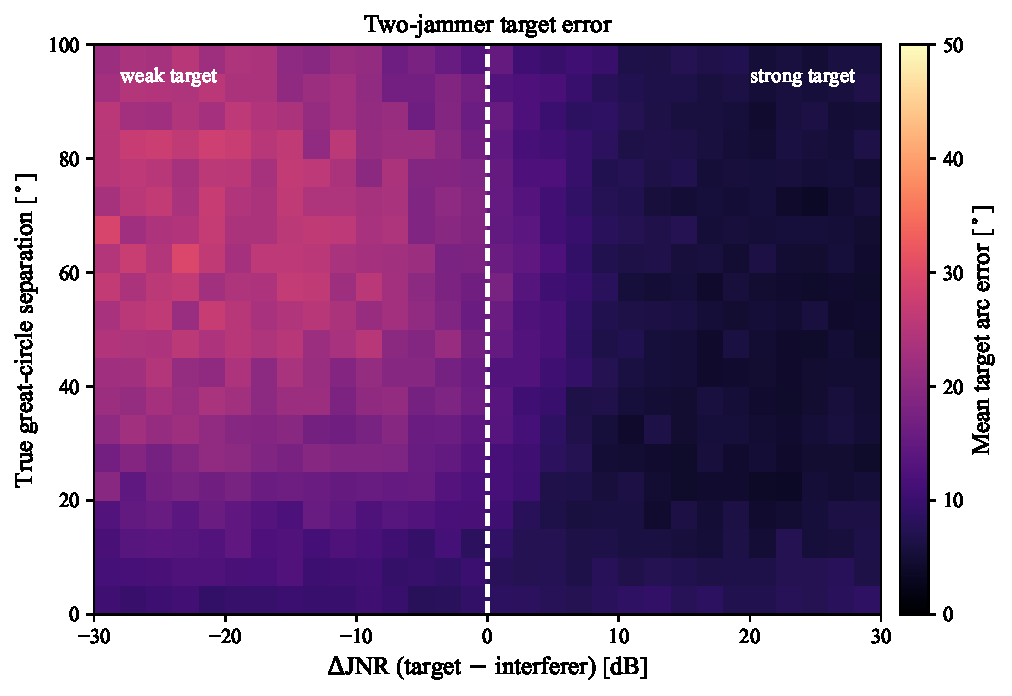
\includegraphics[width=\columnwidth]{phase3_5_error_heatmap}
\caption{Error over the joint space of the two jammers' directions and powers
(PH35). The evaluation split populates only $\drEvalPop\%$ of cells at the
five-sample threshold, so the map is also drawn on a synthesised grid of
$\drGridScenes$ scenes retained from $\drGridDrawn$ draws, which fills every
cell. With the grid complete, an empty cell means a geometry the physics does
not permit rather than one the sampler happened to miss.}
\label{fig:drmap}
\end{figure}

One methodological point travels with Fig.~\ref{fig:drmap}. On the evaluation
split only $\drEvalPop\%$ of the cells of the joint direction/power map reach
the five-sample threshold, which makes an empty cell ambiguous: it may be a
geometry that cannot occur, or merely one the random sampler did not visit. We
therefore redrew the map on a purpose-built grid, retaining $\drGridScenes$
scenes from $\drGridDrawn$ draws, which populates every cell. Only then can a
blank region be read as a physical statement.

\section{From Direction to Suppression}
\label{sec:jsr}

Direction error is an intermediate quantity. What a receiver experiences is the
jammer-to-signal ratio after nulling, and that is what this section reports.
Estimated directions are turned into weights by the projection nulling of
\eqref{eq:projnull}, and the resulting $\JSR$ of \eqref{eq:jsr} is evaluated
against the same full-wave patterns used to generate the measurement. The
figure is clipped at a $\jsrCap\dB$ ceiling and floored at zero, so what is
reported is deliberately conservative: no scene is credited with more
suppression than a real front end would deliver.

\subsection{Single Jammer}
\label{sec:jsr:one}

Over $\jsrN$ single-jammer scenes, with no scene discarded as degenerate, the
median $\JSR$ is $\jsrMed\dB$, with a tenth percentile of $\jsrPten\dB$ and a
ninetieth of $\jsrPninety\dB$. Expressed as coverage, $\pJsrTen\%$ of scenes
achieve at least $10\dB$ of suppression, $\pJsrTwenty\%$ at least $20\dB$, and
$\pJsrThirty\%$ at least $30\dB$. The tenth percentile is the number an
integrator should plan against, and it is comfortably above the threshold at
which a GNSS receiver recovers lock.

\begin{figure}[!t]
\centering
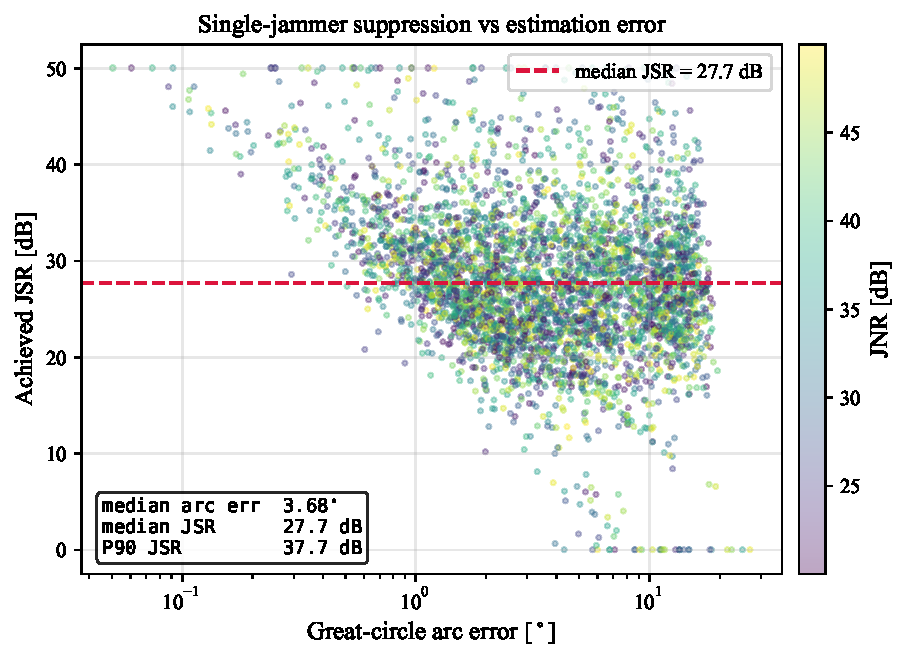
\includegraphics[width=\columnwidth]{phase4_jsr_vs_error}
\caption{Suppression against direction error over $\jsrN$ single-jammer scenes
(PH4). The relationship is strikingly flat: the median $\JSR$ falls only from
$\jsrErrOne\dB$ for scenes accurate to within $1\degs$ to $\jsrErrFive\dB$ for
scenes accurate to within $5\degs$. A null cast by a $\apertureLambda\lambda$
aperture is broad, so the suppression tolerates a direction error of several
degrees almost without penalty.}
\label{fig:jsrerr}
\end{figure}

Fig.~\ref{fig:jsrerr} makes the operationally important point. Conditioning on
direction accuracy, the median $\JSR$ is $\jsrErrOne\dB$ for scenes with arc
error within $1\degs$ ($n = \nJsrErrOne$), $\jsrErrThree\dB$ within $3\degs$
($n = \nJsrErrThree$), and $\jsrErrFive\dB$ within $5\degs$
($n = \nJsrErrFive$). A fivefold relaxation of the accuracy requirement costs
about $6\dB$. The explanation is the aperture: a null formed on
$\apertureLambda\lambda$ is angularly broad, so the pattern null does not have
to be placed precisely to place the jammer deep inside it. This is why a
median direction error of $\netArcPfifty\degs$ is not merely acceptable but
close to sufficient, and it is the reason a modest estimator on a small array
remains useful.

\subsection{Two and Three Jammers}
\label{sec:jsr:multi}

With two jammers the dynamic-range asymmetry of
Section~\ref{sec:dynrange} propagates straight through to suppression. Over
$\jsrN$ two-jammer scenes, evaluated once per jammer, the mean $\JSR$ is
$\jsrTwoJstrong\dB$ for the stronger jammer and $\jsrTwoJweak\dB$ for the
weaker one. The weaker jammer is both harder to locate and, having been located
poorly, less well nulled.

Splitting instead by geometry gives a result that reads backwards at first
sight: widely separated pairs, at least $60\degs$ apart, average
$\jsrSepFar\dB$, while closely spaced pairs under $30\degs$ average
$\jsrSepNear\dB$. Closer jammers are suppressed \emph{better}. The likely
mechanism is that two nulls demanded of an $\numElem$-element array consume
both spare degrees of freedom when the directions are far apart, and each must
then be placed accurately on its own target; when the two directions are close,
a single broad null covers both, and the direction errors --- which are
correlated in that regime --- move the pair together inside a null wide enough
to hold them. We offer this as the most plausible reading of the measurement
rather than as a demonstrated mechanism; separating the two contributions would
require an ablation we have not run.

\begin{figure}[!t]
\centering
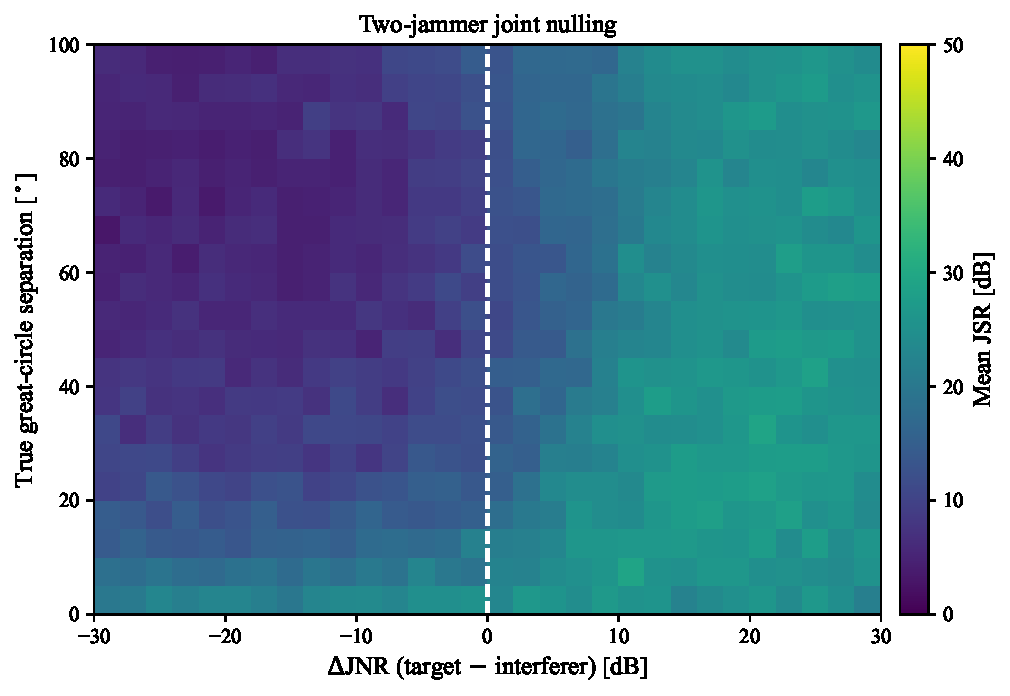
\includegraphics[width=\columnwidth]{phase4_2_jsr_heatmap}
\caption{Two-jammer suppression over the joint direction/power space (PH4). As
in Fig.~\ref{fig:drmap}, the evaluation split reaches the five-sample threshold
in only $\jsrHeatEval\%$ of cells, so the map is redrawn on the synthesised
grid, where every cell is populated and the weak/strong means are
$\jsrTwoJgridWeak\dB$ and $\jsrTwoJgridStrong\dB$.}
\label{fig:jsrmap}
\end{figure}

Three jammers are reported for completeness and should be read as a feasibility
check. Over $\nThreeJnull$ scenes, with no degenerate geometry encountered, the
mean $\JSR$ is $\jsrThreeJmean\dB$ and the median $\jsrThreeJmed\dB$, with
$\pJsrThreeJten\%$ of scenes reaching $10\dB$. The limitation is structural
rather than algorithmic: casting three nulls with $\numElem$ elements leaves a
single degree of freedom for everything else, so even exact directions would
purchase only limited quiescent gain. Improving this number requires more
elements, not a better estimator.

\section{Discussion and Limitations}
\label{sec:disc}

The results support a narrow claim, and it is worth stating what the claim does
and does not include.

\emph{The sector index is an input.} Every result in this paper is conditioned
on knowing which of the $\numSectors$ sectors is being queried, because the
codebook is per-sector. Acquisition of the sector --- scanning the sectors, or
fusing their probe vectors --- is outside the scope of this work. A full system
would either sweep all $\numSectors$ sectors, multiplying the
$0.40\,\mathrm{s}$ scan time of Section~\ref{sec:model:stats} accordingly, or
use a coarse omnidirectional detector to select one. We consider this the most
significant gap between what is measured here and a deployable receiver.

\emph{The elevation split does double duty.} The band boundary at
$\theta = \elevSplit\degs$ is simultaneously the equal-solid-angle split and a
codebook boundary. Every elevation-resolved result therefore mixes a geometric
effect with a boundary effect, and we have flagged this wherever such a result
appears. Disentangling the two requires a second codebook with the split moved,
which we have not built.

\emph{The array is simulated, not measured.} The element patterns are full-wave
simulations of the mounted array, which captures pattern diversity and mutual
coupling as modelled, but not manufacturing tolerance, mounting variation or
calibration error. The observability argument of
Section~\ref{sec:bounds:ceiling} depends on pattern diversity being real, and
that dependence should be validated on hardware before the $J \le \jIdent$
ceiling is relied upon in a design.

\emph{The bound is not the right yardstick, and we do not claim to beat it.}
The estimator is measurably biased toward subsector centres. On
ill-conditioned geometries its RMSE falls below the unbiased Cram\'er--Rao
bound, and Section~\ref{sec:single:bias} shows by direct measurement that those
cells are bias-dominated: the bias grows by $\fdBiasGrowth$ between the
conditioning halves while the scatter moves by $\fdScatGrowth\%$. A biased
estimator is not governed by the unbiased bound, so the sub-bound cells are a
statement about our estimator's class, not an achievement. No claim of bound
violation is made anywhere in this paper.

\emph{Dynamic range is the dominant weakness.} The plateau of
Section~\ref{sec:dynrange} means a target buried more than about
$\drPlateauOnset\dB$ below its interferer is answered at sector scale, roughly
$\sectorRadius\degs$, rather than tracked. Graceful degradation is preferable
to divergence, but it is not detection, and this is the first thing we would
attack in future work.

\emph{The jammer count is assumed known.} Results are reported at fixed $J$.
Estimating $J$ from the probe vector is a natural extension and is made
plausible by the observability accounting of
Section~\ref{sec:bounds:ceiling}, but it is not attempted here.

\section{Conclusion}
\label{sec:concl}

An analog CRPA that reports only $\numProbes$ scalar powers per sector query
carries enough information to steer nulls onto multiple jammers in real time.
We made that statement precise in three steps. First, the observable content of
any power-only scan of an $\numElem$-element array is bounded by the
$\dObs$ real dimensions of the spatial covariance, which caps joint
identifiability at $J \le \jIdent$ and shows the widely quoted limit of
$\jIdentIdeal$ jammers to be an artifact of the common-element-pattern
idealisation rather than a property of a real mounted array. Second, we derived
the Fisher information of the measurement in the form the hardware actually
delivers it and verified it against the generator, which supplies a per-scene
bound and, more usefully, a per-scene conditioning number that predicts where
the problem is hard. Third, we built a $\modelParams$-parameter estimator
whose output lies in the upper hemisphere by construction and which reads the
notch structure of the codebook directly, reaching a median arc error of
$\netArcPfifty\degs$ on single jammers and delivering a median
$\jsrMed\dB$ of suppression after projection nulling, with $\pJsrTwenty\%$ of
scenes above $20\dB$.

The diagnostic results are as much of the contribution as the accuracy
figures. Efficiency relative to the bound is not a number for this problem but
a function of geometry, $\effWell$ on well-conditioned scenes and $\effIll$ on
ill-conditioned ones; a fixed-direction experiment shows the sub-bound cells to
be bias-dominated, with the bias pointing inward toward the subsector centres
the anchor is built from; and the dynamic-range sweep shows the estimator
abandoning the weak-source law entirely in favour of a sector-scale fallback.
Each of these is a property of an estimator that has been given a strong
geometric prior, and each of them tells a designer something the aggregate
accuracy figures conceal. The immediate next steps follow from the limitations:
sector acquisition, a dynamic-range-aware codebook or a two-pass scan, and
validation of the pattern-diversity argument on measured hardware.
\bibliographystyle{IEEEtran}
\bibliography{references}

\end{document}

